\documentclass[twoside]{book}

% Packages required by doxygen
\usepackage{fixltx2e}
\usepackage{calc}
\usepackage{doxygen}
\usepackage[export]{adjustbox} % also loads graphicx
\usepackage{graphicx}
\usepackage[utf8]{inputenc}
\usepackage{makeidx}
\usepackage{multicol}
\usepackage{multirow}
\PassOptionsToPackage{warn}{textcomp}
\usepackage{textcomp}
\usepackage[nointegrals]{wasysym}
\usepackage[table]{xcolor}

% Font selection
\usepackage[T1]{fontenc}
\usepackage[scaled=.90]{helvet}
\usepackage{courier}
\usepackage{amssymb}
\usepackage{sectsty}
\renewcommand{\familydefault}{\sfdefault}
\allsectionsfont{%
  \fontseries{bc}\selectfont%
  \color{darkgray}%
}
\renewcommand{\DoxyLabelFont}{%
  \fontseries{bc}\selectfont%
  \color{darkgray}%
}
\newcommand{\+}{\discretionary{\mbox{\scriptsize$\hookleftarrow$}}{}{}}

% Page & text layout
\usepackage{geometry}
\geometry{%
  a4paper,%
  top=2.5cm,%
  bottom=2.5cm,%
  left=2.5cm,%
  right=2.5cm%
}
\tolerance=750
\hfuzz=15pt
\hbadness=750
\setlength{\emergencystretch}{15pt}
\setlength{\parindent}{0cm}
\setlength{\parskip}{3ex plus 2ex minus 2ex}
\makeatletter
\renewcommand{\paragraph}{%
  \@startsection{paragraph}{4}{0ex}{-1.0ex}{1.0ex}{%
    \normalfont\normalsize\bfseries\SS@parafont%
  }%
}
\renewcommand{\subparagraph}{%
  \@startsection{subparagraph}{5}{0ex}{-1.0ex}{1.0ex}{%
    \normalfont\normalsize\bfseries\SS@subparafont%
  }%
}
\makeatother

% Headers & footers
\usepackage{fancyhdr}
\pagestyle{fancyplain}
\fancyhead[LE]{\fancyplain{}{\bfseries\thepage}}
\fancyhead[CE]{\fancyplain{}{}}
\fancyhead[RE]{\fancyplain{}{\bfseries\leftmark}}
\fancyhead[LO]{\fancyplain{}{\bfseries\rightmark}}
\fancyhead[CO]{\fancyplain{}{}}
\fancyhead[RO]{\fancyplain{}{\bfseries\thepage}}
\fancyfoot[LE]{\fancyplain{}{}}
\fancyfoot[CE]{\fancyplain{}{}}
\fancyfoot[RE]{\fancyplain{}{\bfseries\scriptsize Generated by Doxygen }}
\fancyfoot[LO]{\fancyplain{}{\bfseries\scriptsize Generated by Doxygen }}
\fancyfoot[CO]{\fancyplain{}{}}
\fancyfoot[RO]{\fancyplain{}{}}
\renewcommand{\footrulewidth}{0.4pt}
\renewcommand{\chaptermark}[1]{%
  \markboth{#1}{}%
}
\renewcommand{\sectionmark}[1]{%
  \markright{\thesection\ #1}%
}

% Indices & bibliography
\usepackage{natbib}
\usepackage[titles]{tocloft}
\setcounter{tocdepth}{3}
\setcounter{secnumdepth}{5}
\makeindex

% Hyperlinks (required, but should be loaded last)
\usepackage{ifpdf}
\ifpdf
  \usepackage[pdftex,pagebackref=true]{hyperref}
\else
  \usepackage[ps2pdf,pagebackref=true]{hyperref}
\fi
\hypersetup{%
  colorlinks=true,%
  linkcolor=blue,%
  citecolor=blue,%
  unicode%
}

% Custom commands
\newcommand{\clearemptydoublepage}{%
  \newpage{\pagestyle{empty}\cleardoublepage}%
}

\usepackage{caption}
\captionsetup{labelsep=space,justification=centering,font={bf},singlelinecheck=off,skip=4pt,position=top}

%===== C O N T E N T S =====

\begin{document}

% Titlepage & ToC
\hypersetup{pageanchor=false,
             bookmarksnumbered=true,
             pdfencoding=unicode
            }
\pagenumbering{alph}
\begin{titlepage}
\vspace*{7cm}
\begin{center}%
{\Large Projecto 1 -\/ A\+E\+DA }\\
\vspace*{1cm}
{\large Generated by Doxygen 1.8.12}\\
\end{center}
\end{titlepage}
\clearemptydoublepage
\pagenumbering{roman}
\tableofcontents
\clearemptydoublepage
\pagenumbering{arabic}
\hypersetup{pageanchor=true}

%--- Begin generated contents ---
\chapter{Hierarchical Index}
\section{Class Hierarchy}
This inheritance list is sorted roughly, but not completely, alphabetically\+:\begin{DoxyCompactList}
\item \contentsline{section}{Bolsa}{\pageref{class_bolsa}}{}
\item \contentsline{section}{Cliente}{\pageref{class_cliente}}{}
\item \contentsline{section}{Data}{\pageref{class_data}}{}
\item \contentsline{section}{Ficheiro\+Inexistente}{\pageref{class_ficheiro_inexistente}}{}
\item \contentsline{section}{Ficheiro\+Invalido}{\pageref{class_ficheiro_invalido}}{}
\item \contentsline{section}{Ordem}{\pageref{class_ordem}}{}
\begin{DoxyCompactList}
\item \contentsline{section}{Ordem\+Compra}{\pageref{class_ordem_compra}}{}
\item \contentsline{section}{Ordem\+Venda}{\pageref{class_ordem_venda}}{}
\end{DoxyCompactList}
\item \contentsline{section}{Transacao}{\pageref{class_transacao}}{}
\end{DoxyCompactList}

\chapter{Class Index}
\section{Class List}
Here are the classes, structs, unions and interfaces with brief descriptions\+:\begin{DoxyCompactList}
\item\contentsline{section}{\hyperlink{class_bolsa}{Bolsa} \\*Classe que guarda os clientes, ordens de compra e venda, e transacoes da bolsa e as funcoes para manipulacao da mesma }{\pageref{class_bolsa}}{}
\item\contentsline{section}{\hyperlink{class_cliente}{Cliente} \\*Classe que guarda o nome e o nif do cliente e as funcoes para manipulacao da mesma }{\pageref{class_cliente}}{}
\item\contentsline{section}{\hyperlink{class_data}{Data} \\*Classe que guarda o dia, mes e ano e as funcoes para manipulacao da mesma }{\pageref{class_data}}{}
\item\contentsline{section}{\hyperlink{class_ficheiro_inexistente}{Ficheiro\+Inexistente} \\*Excecao que e lancada quando se tenta abrir um ficheiro inexistente }{\pageref{class_ficheiro_inexistente}}{}
\item\contentsline{section}{\hyperlink{class_ficheiro_invalido}{Ficheiro\+Invalido} \\*Excecao que e lancada quando se abre um ficheiro invalido }{\pageref{class_ficheiro_invalido}}{}
\item\contentsline{section}{\hyperlink{class_ordem}{Ordem} \\*Classe que representa uma ordem na bolsa de valores }{\pageref{class_ordem}}{}
\item\contentsline{section}{\hyperlink{class_ordem_compra}{Ordem\+Compra} \\*Classe que representa uma ordem de compra na bolsa de valores }{\pageref{class_ordem_compra}}{}
\item\contentsline{section}{\hyperlink{class_ordem_venda}{Ordem\+Venda} \\*Classe que representa uma ordem de venda na bolsa de valores }{\pageref{class_ordem_venda}}{}
\item\contentsline{section}{\hyperlink{class_transacao}{Transacao} \\*Classe que representa uma transacao na bolsa de valores }{\pageref{class_transacao}}{}
\end{DoxyCompactList}

\chapter{File Index}
\section{File List}
Here is a list of all files with brief descriptions\+:\begin{DoxyCompactList}
\item\contentsline{section}{\hyperlink{_bolsa_8cpp}{Bolsa.\+cpp} }{\pageref{_bolsa_8cpp}}{}
\item\contentsline{section}{\hyperlink{_bolsa_8h}{Bolsa.\+h} }{\pageref{_bolsa_8h}}{}
\item\contentsline{section}{\hyperlink{_cliente_8cpp}{Cliente.\+cpp} }{\pageref{_cliente_8cpp}}{}
\item\contentsline{section}{\hyperlink{_cliente_8h}{Cliente.\+h} }{\pageref{_cliente_8h}}{}
\item\contentsline{section}{\hyperlink{_data_8cpp}{Data.\+cpp} }{\pageref{_data_8cpp}}{}
\item\contentsline{section}{\hyperlink{_data_8h}{Data.\+h} }{\pageref{_data_8h}}{}
\item\contentsline{section}{\hyperlink{_excecoes_8cpp}{Excecoes.\+cpp} }{\pageref{_excecoes_8cpp}}{}
\item\contentsline{section}{\hyperlink{_excecoes_8h}{Excecoes.\+h} }{\pageref{_excecoes_8h}}{}
\item\contentsline{section}{\hyperlink{insertion_sort_8h}{insertion\+Sort.\+h} }{\pageref{insertion_sort_8h}}{}
\item\contentsline{section}{\hyperlink{main_8cpp}{main.\+cpp} }{\pageref{main_8cpp}}{}
\item\contentsline{section}{\hyperlink{_menus_8cpp}{Menus.\+cpp} }{\pageref{_menus_8cpp}}{}
\item\contentsline{section}{\hyperlink{_menus_8h}{Menus.\+h} }{\pageref{_menus_8h}}{}
\item\contentsline{section}{\hyperlink{_ordem_8cpp}{Ordem.\+cpp} }{\pageref{_ordem_8cpp}}{}
\item\contentsline{section}{\hyperlink{_ordem_8h}{Ordem.\+h} }{\pageref{_ordem_8h}}{}
\item\contentsline{section}{\hyperlink{_ordem_compra_8cpp}{Ordem\+Compra.\+cpp} }{\pageref{_ordem_compra_8cpp}}{}
\item\contentsline{section}{\hyperlink{_ordem_compra_8h}{Ordem\+Compra.\+h} }{\pageref{_ordem_compra_8h}}{}
\item\contentsline{section}{\hyperlink{_ordem_venda_8cpp}{Ordem\+Venda.\+cpp} }{\pageref{_ordem_venda_8cpp}}{}
\item\contentsline{section}{\hyperlink{_ordem_venda_8h}{Ordem\+Venda.\+h} }{\pageref{_ordem_venda_8h}}{}
\item\contentsline{section}{\hyperlink{_transacao_8cpp}{Transacao.\+cpp} }{\pageref{_transacao_8cpp}}{}
\item\contentsline{section}{\hyperlink{_transacao_8h}{Transacao.\+h} }{\pageref{_transacao_8h}}{}
\item\contentsline{section}{\hyperlink{_utils_8cpp}{Utils.\+cpp} }{\pageref{_utils_8cpp}}{}
\item\contentsline{section}{\hyperlink{_utils_8h}{Utils.\+h} }{\pageref{_utils_8h}}{}
\end{DoxyCompactList}

\chapter{Class Documentation}
\hypertarget{class_bolsa}{}\section{Bolsa Class Reference}
\label{class_bolsa}\index{Bolsa@{Bolsa}}


Classe que guarda os clientes, ordens de compra e venda, e transacoes da bolsa e as funcoes para manipulacao da mesma.  




{\ttfamily \#include $<$Bolsa.\+h$>$}

\subsection*{Public Member Functions}
\begin{DoxyCompactItemize}
\item 
\hyperlink{class_bolsa_a79eb058719d17c21fab6c4b95db8c1b6}{Bolsa} ()
\begin{DoxyCompactList}\small\item\em Construtor por defeito. \end{DoxyCompactList}\item 
void \hyperlink{class_bolsa_aabb97dba1ba1783fbe860058764c6a90}{le\+\_\+ficheiros} (string \&\hyperlink{_utils_8h_a1335b18f135ed58c716b3ddcecdc8cce}{fich\+Clientes}, string \&\hyperlink{_utils_8h_a66ff7fedd13a1b40664042a086ca0f27}{fich\+Transacoes}, string \&\hyperlink{_utils_8h_ad22902af7efe6d185550055b7caa5cbb}{fich\+Ordens\+Venda}, string \&\hyperlink{_utils_8h_acaee3ba642d3be244820a97e5eb5b7f7}{fich\+Ordens\+Compra})
\begin{DoxyCompactList}\small\item\em Le os ficheiros com informacoes para preencher os vectores da bolsa. \end{DoxyCompactList}\item 
void \hyperlink{class_bolsa_a2f295e1c0ddd43401056bde7d6a9bfde}{le\+\_\+ficheiros\+\_\+cli} (string \&\hyperlink{_utils_8h_a1335b18f135ed58c716b3ddcecdc8cce}{fich\+Clientes})
\begin{DoxyCompactList}\small\item\em Le o ficheiro com as informacoes dos clientes. \end{DoxyCompactList}\item 
void \hyperlink{class_bolsa_ab099261f63bff9e274b94bca96cbd2f4}{le\+\_\+ficheiros\+\_\+tran} (string \&\hyperlink{_utils_8h_a66ff7fedd13a1b40664042a086ca0f27}{fich\+Transacoes})
\begin{DoxyCompactList}\small\item\em Le o ficheiro com as informacoes das transacoes. \end{DoxyCompactList}\item 
void \hyperlink{class_bolsa_ab0cd2fab3d7490d5d4a431e5cb1106e6}{le\+\_\+ficheiros\+\_\+ordv} (string \&\hyperlink{_utils_8h_ad22902af7efe6d185550055b7caa5cbb}{fich\+Ordens\+Venda})
\begin{DoxyCompactList}\small\item\em Le o ficheiro com as informacoes das ordens de venda. \end{DoxyCompactList}\item 
void \hyperlink{class_bolsa_a57e3864eac22b2690e04fb8be39b5e58}{le\+\_\+ficheiros\+\_\+ordc} (string \&\hyperlink{_utils_8h_acaee3ba642d3be244820a97e5eb5b7f7}{fich\+Ordens\+Compra})
\begin{DoxyCompactList}\small\item\em Le o ficheiro com as informacoes das ordens de compra. \end{DoxyCompactList}\item 
void \hyperlink{class_bolsa_a12c0a8faf58b0803228ed17022c6ecfe}{guarda\+\_\+alteracoes} (int n, string \&fich)
\begin{DoxyCompactList}\small\item\em Guarda alteracoes feitas nos vectores no ficheiro fich. \end{DoxyCompactList}\item 
void \hyperlink{class_bolsa_a6567e62d4d1037ca2e2263ba7e22ea4e}{ad\+\_\+ordem\+\_\+compra} ()
\begin{DoxyCompactList}\small\item\em Adiciona uma ordem de compra ao vector de ordens de compra, com parametros definidos pelo utilizador. \end{DoxyCompactList}\item 
void \hyperlink{class_bolsa_ab028d3fd8537fa65b25c7eece82dfabc}{ad\+\_\+ordem\+\_\+venda} ()
\begin{DoxyCompactList}\small\item\em Adiciona uma ordem de venda ao vector de ordens de venda, com parametros definidos pelo utilizador. \end{DoxyCompactList}\item 
void \hyperlink{class_bolsa_a8bcc217341ffe40e4f2b6d7454977d4d}{ad\+\_\+cli} ()
\begin{DoxyCompactList}\small\item\em Adiciona um cliente ao vector de clientes, com parametros definidos pelo utilizador. \end{DoxyCompactList}\item 
void \hyperlink{class_bolsa_a831836b62c66324d7eaf4c71a4e8015e}{rem\+\_\+ordem\+\_\+compra} ()
\begin{DoxyCompactList}\small\item\em Remove uma ordem de compra ao vector de ordens de compra, com parametros definidos pelo utilizador. \end{DoxyCompactList}\item 
void \hyperlink{class_bolsa_a293578d28d9de84f85844025b47fc505}{rem\+\_\+ordem\+\_\+venda} ()
\begin{DoxyCompactList}\small\item\em Remove uma ordem de venda do vector de ordens de venda, com parametros definidos pelo utilizador. \end{DoxyCompactList}\item 
void \hyperlink{class_bolsa_a3fe70cc3887113b99e09457a62d3fb83}{rem\+\_\+cli} ()
\begin{DoxyCompactList}\small\item\em Remove um cliente do vector de clientes, com parametros definidos pelo utilizador. \end{DoxyCompactList}\item 
void \hyperlink{class_bolsa_a4676ec9295a14426f3c70e91dd36fde1}{listar\+\_\+transacoes} ()
\begin{DoxyCompactList}\small\item\em sdsddddddddddddssadsaads \end{DoxyCompactList}\item 
void \hyperlink{class_bolsa_ad96a358bf03c103f55b8139da8a0d61a}{listar\+\_\+transacoes\+\_\+cli} ()
\begin{DoxyCompactList}\small\item\em Lista as transacoes de um cliente. \end{DoxyCompactList}\item 
void \hyperlink{class_bolsa_aeac084d57bf9382c83516f1f0c043936}{listar\+\_\+transacoes\+\_\+titulo} ()
\begin{DoxyCompactList}\small\item\em Lista todas as transacoes com um certo titulo. \end{DoxyCompactList}\item 
void \hyperlink{class_bolsa_acb012fa60aa074fd861168ca3aedadd0}{listar\+\_\+transacoes\+\_\+intervalo\+\_\+de\+\_\+tempo} ()
\begin{DoxyCompactList}\small\item\em Lista transacoes por dia, mes ou ano. \end{DoxyCompactList}\item 
void \hyperlink{class_bolsa_aba662f57e78213bee6de3db7c06c7293}{listar\+\_\+clientes} ()
\begin{DoxyCompactList}\small\item\em Lista todos os clientes. \end{DoxyCompactList}\item 
void \hyperlink{class_bolsa_abd28d5b93c338a05deccf0adbac23ba1}{listar\+\_\+ordens\+Venda} ()
\begin{DoxyCompactList}\small\item\em Lista todas as de ordens venda. \end{DoxyCompactList}\item 
void \hyperlink{class_bolsa_a419cf3df5db87b4925eb616af1180f88}{listar\+\_\+ordens\+Compra} ()
\begin{DoxyCompactList}\small\item\em Lista todas as de ordens compra. \end{DoxyCompactList}\end{DoxyCompactItemize}


\subsection{Detailed Description}
Classe que guarda os clientes, ordens de compra e venda, e transacoes da bolsa e as funcoes para manipulacao da mesma. 

\subsection{Constructor \& Destructor Documentation}
\hypertarget{class_bolsa_a79eb058719d17c21fab6c4b95db8c1b6}{}\label{class_bolsa_a79eb058719d17c21fab6c4b95db8c1b6} 
\index{Bolsa@{Bolsa}!Bolsa@{Bolsa}}
\index{Bolsa@{Bolsa}!Bolsa@{Bolsa}}
\subsubsection{\texorpdfstring{Bolsa()}{Bolsa()}}
{\footnotesize\ttfamily Bolsa\+::\+Bolsa (\begin{DoxyParamCaption}{ }\end{DoxyParamCaption})\hspace{0.3cm}{\ttfamily [inline]}}



Construtor por defeito. 



\subsection{Member Function Documentation}
\hypertarget{class_bolsa_a8bcc217341ffe40e4f2b6d7454977d4d}{}\label{class_bolsa_a8bcc217341ffe40e4f2b6d7454977d4d} 
\index{Bolsa@{Bolsa}!ad\+\_\+cli@{ad\+\_\+cli}}
\index{ad\+\_\+cli@{ad\+\_\+cli}!Bolsa@{Bolsa}}
\subsubsection{\texorpdfstring{ad\+\_\+cli()}{ad\_cli()}}
{\footnotesize\ttfamily void Bolsa\+::ad\+\_\+cli (\begin{DoxyParamCaption}{ }\end{DoxyParamCaption})}



Adiciona um cliente ao vector de clientes, com parametros definidos pelo utilizador. 

\hypertarget{class_bolsa_a6567e62d4d1037ca2e2263ba7e22ea4e}{}\label{class_bolsa_a6567e62d4d1037ca2e2263ba7e22ea4e} 
\index{Bolsa@{Bolsa}!ad\+\_\+ordem\+\_\+compra@{ad\+\_\+ordem\+\_\+compra}}
\index{ad\+\_\+ordem\+\_\+compra@{ad\+\_\+ordem\+\_\+compra}!Bolsa@{Bolsa}}
\subsubsection{\texorpdfstring{ad\+\_\+ordem\+\_\+compra()}{ad\_ordem\_compra()}}
{\footnotesize\ttfamily void Bolsa\+::ad\+\_\+ordem\+\_\+compra (\begin{DoxyParamCaption}{ }\end{DoxyParamCaption})}



Adiciona uma ordem de compra ao vector de ordens de compra, com parametros definidos pelo utilizador. 

\hypertarget{class_bolsa_ab028d3fd8537fa65b25c7eece82dfabc}{}\label{class_bolsa_ab028d3fd8537fa65b25c7eece82dfabc} 
\index{Bolsa@{Bolsa}!ad\+\_\+ordem\+\_\+venda@{ad\+\_\+ordem\+\_\+venda}}
\index{ad\+\_\+ordem\+\_\+venda@{ad\+\_\+ordem\+\_\+venda}!Bolsa@{Bolsa}}
\subsubsection{\texorpdfstring{ad\+\_\+ordem\+\_\+venda()}{ad\_ordem\_venda()}}
{\footnotesize\ttfamily void Bolsa\+::ad\+\_\+ordem\+\_\+venda (\begin{DoxyParamCaption}{ }\end{DoxyParamCaption})}



Adiciona uma ordem de venda ao vector de ordens de venda, com parametros definidos pelo utilizador. 

\hypertarget{class_bolsa_a12c0a8faf58b0803228ed17022c6ecfe}{}\label{class_bolsa_a12c0a8faf58b0803228ed17022c6ecfe} 
\index{Bolsa@{Bolsa}!guarda\+\_\+alteracoes@{guarda\+\_\+alteracoes}}
\index{guarda\+\_\+alteracoes@{guarda\+\_\+alteracoes}!Bolsa@{Bolsa}}
\subsubsection{\texorpdfstring{guarda\+\_\+alteracoes()}{guarda\_alteracoes()}}
{\footnotesize\ttfamily void Bolsa\+::guarda\+\_\+alteracoes (\begin{DoxyParamCaption}\item[{int}]{n,  }\item[{string \&}]{fich }\end{DoxyParamCaption})}



Guarda alteracoes feitas nos vectores no ficheiro fich. 


\begin{DoxyParams}{Parameters}
{\em n} & Inteiro de 1 a 4 que representa os varios vectores da bolsa. \\
\hline
{\em fich} & O ficheiro onde o vector e guardado. \\
\hline
\end{DoxyParams}
\hypertarget{class_bolsa_aabb97dba1ba1783fbe860058764c6a90}{}\label{class_bolsa_aabb97dba1ba1783fbe860058764c6a90} 
\index{Bolsa@{Bolsa}!le\+\_\+ficheiros@{le\+\_\+ficheiros}}
\index{le\+\_\+ficheiros@{le\+\_\+ficheiros}!Bolsa@{Bolsa}}
\subsubsection{\texorpdfstring{le\+\_\+ficheiros()}{le\_ficheiros()}}
{\footnotesize\ttfamily void Bolsa\+::le\+\_\+ficheiros (\begin{DoxyParamCaption}\item[{string \&}]{fich\+Clientes,  }\item[{string \&}]{fich\+Transacoes,  }\item[{string \&}]{fich\+Ordens\+Venda,  }\item[{string \&}]{fich\+Ordens\+Compra }\end{DoxyParamCaption})}



Le os ficheiros com informacoes para preencher os vectores da bolsa. 


\begin{DoxyParams}{Parameters}
{\em fich\+Clientes} & Ficheiro com as informacoes dos clientes. \\
\hline
{\em fich\+Transacoes} & Ficheiro com as informacoes das transacoes. \\
\hline
{\em fich\+Ordens\+Venda} & Ficheiro com as informacoes das ordens venda. \\
\hline
{\em fich\+Ordens\+Compra} & Ficheiro com as informacoes das ordens compra. \\
\hline
\end{DoxyParams}
\hypertarget{class_bolsa_a2f295e1c0ddd43401056bde7d6a9bfde}{}\label{class_bolsa_a2f295e1c0ddd43401056bde7d6a9bfde} 
\index{Bolsa@{Bolsa}!le\+\_\+ficheiros\+\_\+cli@{le\+\_\+ficheiros\+\_\+cli}}
\index{le\+\_\+ficheiros\+\_\+cli@{le\+\_\+ficheiros\+\_\+cli}!Bolsa@{Bolsa}}
\subsubsection{\texorpdfstring{le\+\_\+ficheiros\+\_\+cli()}{le\_ficheiros\_cli()}}
{\footnotesize\ttfamily void Bolsa\+::le\+\_\+ficheiros\+\_\+cli (\begin{DoxyParamCaption}\item[{string \&}]{fich\+Clientes }\end{DoxyParamCaption})}



Le o ficheiro com as informacoes dos clientes. 


\begin{DoxyParams}{Parameters}
{\em fich\+Clientes} & Ficheiro com as informacoes dos clientes. \\
\hline
\end{DoxyParams}
\hypertarget{class_bolsa_a57e3864eac22b2690e04fb8be39b5e58}{}\label{class_bolsa_a57e3864eac22b2690e04fb8be39b5e58} 
\index{Bolsa@{Bolsa}!le\+\_\+ficheiros\+\_\+ordc@{le\+\_\+ficheiros\+\_\+ordc}}
\index{le\+\_\+ficheiros\+\_\+ordc@{le\+\_\+ficheiros\+\_\+ordc}!Bolsa@{Bolsa}}
\subsubsection{\texorpdfstring{le\+\_\+ficheiros\+\_\+ordc()}{le\_ficheiros\_ordc()}}
{\footnotesize\ttfamily void Bolsa\+::le\+\_\+ficheiros\+\_\+ordc (\begin{DoxyParamCaption}\item[{string \&}]{fich\+Ordens\+Compra }\end{DoxyParamCaption})}



Le o ficheiro com as informacoes das ordens de compra. 


\begin{DoxyParams}{Parameters}
{\em fich\+Ordens\+Compra} & Ficheiro com as informacoes das ordens compra. \\
\hline
\end{DoxyParams}
\hypertarget{class_bolsa_ab0cd2fab3d7490d5d4a431e5cb1106e6}{}\label{class_bolsa_ab0cd2fab3d7490d5d4a431e5cb1106e6} 
\index{Bolsa@{Bolsa}!le\+\_\+ficheiros\+\_\+ordv@{le\+\_\+ficheiros\+\_\+ordv}}
\index{le\+\_\+ficheiros\+\_\+ordv@{le\+\_\+ficheiros\+\_\+ordv}!Bolsa@{Bolsa}}
\subsubsection{\texorpdfstring{le\+\_\+ficheiros\+\_\+ordv()}{le\_ficheiros\_ordv()}}
{\footnotesize\ttfamily void Bolsa\+::le\+\_\+ficheiros\+\_\+ordv (\begin{DoxyParamCaption}\item[{string \&}]{fich\+Ordens\+Venda }\end{DoxyParamCaption})}



Le o ficheiro com as informacoes das ordens de venda. 


\begin{DoxyParams}{Parameters}
{\em fich\+Ordens\+Venda} & Ficheiro com as informacoes das ordens venda. \\
\hline
\end{DoxyParams}
\hypertarget{class_bolsa_ab099261f63bff9e274b94bca96cbd2f4}{}\label{class_bolsa_ab099261f63bff9e274b94bca96cbd2f4} 
\index{Bolsa@{Bolsa}!le\+\_\+ficheiros\+\_\+tran@{le\+\_\+ficheiros\+\_\+tran}}
\index{le\+\_\+ficheiros\+\_\+tran@{le\+\_\+ficheiros\+\_\+tran}!Bolsa@{Bolsa}}
\subsubsection{\texorpdfstring{le\+\_\+ficheiros\+\_\+tran()}{le\_ficheiros\_tran()}}
{\footnotesize\ttfamily void Bolsa\+::le\+\_\+ficheiros\+\_\+tran (\begin{DoxyParamCaption}\item[{string \&}]{fich\+Transacoes }\end{DoxyParamCaption})}



Le o ficheiro com as informacoes das transacoes. 


\begin{DoxyParams}{Parameters}
{\em fich\+Transacoes} & Ficheiro com as informacoes das transacoes. \\
\hline
\end{DoxyParams}
\hypertarget{class_bolsa_aba662f57e78213bee6de3db7c06c7293}{}\label{class_bolsa_aba662f57e78213bee6de3db7c06c7293} 
\index{Bolsa@{Bolsa}!listar\+\_\+clientes@{listar\+\_\+clientes}}
\index{listar\+\_\+clientes@{listar\+\_\+clientes}!Bolsa@{Bolsa}}
\subsubsection{\texorpdfstring{listar\+\_\+clientes()}{listar\_clientes()}}
{\footnotesize\ttfamily void Bolsa\+::listar\+\_\+clientes (\begin{DoxyParamCaption}{ }\end{DoxyParamCaption})}



Lista todos os clientes. 

\hypertarget{class_bolsa_a419cf3df5db87b4925eb616af1180f88}{}\label{class_bolsa_a419cf3df5db87b4925eb616af1180f88} 
\index{Bolsa@{Bolsa}!listar\+\_\+ordens\+Compra@{listar\+\_\+ordens\+Compra}}
\index{listar\+\_\+ordens\+Compra@{listar\+\_\+ordens\+Compra}!Bolsa@{Bolsa}}
\subsubsection{\texorpdfstring{listar\+\_\+ordens\+Compra()}{listar\_ordensCompra()}}
{\footnotesize\ttfamily void Bolsa\+::listar\+\_\+ordens\+Compra (\begin{DoxyParamCaption}{ }\end{DoxyParamCaption})}



Lista todas as de ordens compra. 

\hypertarget{class_bolsa_abd28d5b93c338a05deccf0adbac23ba1}{}\label{class_bolsa_abd28d5b93c338a05deccf0adbac23ba1} 
\index{Bolsa@{Bolsa}!listar\+\_\+ordens\+Venda@{listar\+\_\+ordens\+Venda}}
\index{listar\+\_\+ordens\+Venda@{listar\+\_\+ordens\+Venda}!Bolsa@{Bolsa}}
\subsubsection{\texorpdfstring{listar\+\_\+ordens\+Venda()}{listar\_ordensVenda()}}
{\footnotesize\ttfamily void Bolsa\+::listar\+\_\+ordens\+Venda (\begin{DoxyParamCaption}{ }\end{DoxyParamCaption})}



Lista todas as de ordens venda. 

\hypertarget{class_bolsa_a4676ec9295a14426f3c70e91dd36fde1}{}\label{class_bolsa_a4676ec9295a14426f3c70e91dd36fde1} 
\index{Bolsa@{Bolsa}!listar\+\_\+transacoes@{listar\+\_\+transacoes}}
\index{listar\+\_\+transacoes@{listar\+\_\+transacoes}!Bolsa@{Bolsa}}
\subsubsection{\texorpdfstring{listar\+\_\+transacoes()}{listar\_transacoes()}}
{\footnotesize\ttfamily void Bolsa\+::listar\+\_\+transacoes (\begin{DoxyParamCaption}{ }\end{DoxyParamCaption})}



sdsddddddddddddssadsaads 

Lista as todas as transacoes. \hypertarget{class_bolsa_ad96a358bf03c103f55b8139da8a0d61a}{}\label{class_bolsa_ad96a358bf03c103f55b8139da8a0d61a} 
\index{Bolsa@{Bolsa}!listar\+\_\+transacoes\+\_\+cli@{listar\+\_\+transacoes\+\_\+cli}}
\index{listar\+\_\+transacoes\+\_\+cli@{listar\+\_\+transacoes\+\_\+cli}!Bolsa@{Bolsa}}
\subsubsection{\texorpdfstring{listar\+\_\+transacoes\+\_\+cli()}{listar\_transacoes\_cli()}}
{\footnotesize\ttfamily void Bolsa\+::listar\+\_\+transacoes\+\_\+cli (\begin{DoxyParamCaption}{ }\end{DoxyParamCaption})}



Lista as transacoes de um cliente. 

\hypertarget{class_bolsa_acb012fa60aa074fd861168ca3aedadd0}{}\label{class_bolsa_acb012fa60aa074fd861168ca3aedadd0} 
\index{Bolsa@{Bolsa}!listar\+\_\+transacoes\+\_\+intervalo\+\_\+de\+\_\+tempo@{listar\+\_\+transacoes\+\_\+intervalo\+\_\+de\+\_\+tempo}}
\index{listar\+\_\+transacoes\+\_\+intervalo\+\_\+de\+\_\+tempo@{listar\+\_\+transacoes\+\_\+intervalo\+\_\+de\+\_\+tempo}!Bolsa@{Bolsa}}
\subsubsection{\texorpdfstring{listar\+\_\+transacoes\+\_\+intervalo\+\_\+de\+\_\+tempo()}{listar\_transacoes\_intervalo\_de\_tempo()}}
{\footnotesize\ttfamily void Bolsa\+::listar\+\_\+transacoes\+\_\+intervalo\+\_\+de\+\_\+tempo (\begin{DoxyParamCaption}{ }\end{DoxyParamCaption})}



Lista transacoes por dia, mes ou ano. 

\hypertarget{class_bolsa_aeac084d57bf9382c83516f1f0c043936}{}\label{class_bolsa_aeac084d57bf9382c83516f1f0c043936} 
\index{Bolsa@{Bolsa}!listar\+\_\+transacoes\+\_\+titulo@{listar\+\_\+transacoes\+\_\+titulo}}
\index{listar\+\_\+transacoes\+\_\+titulo@{listar\+\_\+transacoes\+\_\+titulo}!Bolsa@{Bolsa}}
\subsubsection{\texorpdfstring{listar\+\_\+transacoes\+\_\+titulo()}{listar\_transacoes\_titulo()}}
{\footnotesize\ttfamily void Bolsa\+::listar\+\_\+transacoes\+\_\+titulo (\begin{DoxyParamCaption}{ }\end{DoxyParamCaption})}



Lista todas as transacoes com um certo titulo. 

\hypertarget{class_bolsa_a3fe70cc3887113b99e09457a62d3fb83}{}\label{class_bolsa_a3fe70cc3887113b99e09457a62d3fb83} 
\index{Bolsa@{Bolsa}!rem\+\_\+cli@{rem\+\_\+cli}}
\index{rem\+\_\+cli@{rem\+\_\+cli}!Bolsa@{Bolsa}}
\subsubsection{\texorpdfstring{rem\+\_\+cli()}{rem\_cli()}}
{\footnotesize\ttfamily void Bolsa\+::rem\+\_\+cli (\begin{DoxyParamCaption}{ }\end{DoxyParamCaption})}



Remove um cliente do vector de clientes, com parametros definidos pelo utilizador. 

\hypertarget{class_bolsa_a831836b62c66324d7eaf4c71a4e8015e}{}\label{class_bolsa_a831836b62c66324d7eaf4c71a4e8015e} 
\index{Bolsa@{Bolsa}!rem\+\_\+ordem\+\_\+compra@{rem\+\_\+ordem\+\_\+compra}}
\index{rem\+\_\+ordem\+\_\+compra@{rem\+\_\+ordem\+\_\+compra}!Bolsa@{Bolsa}}
\subsubsection{\texorpdfstring{rem\+\_\+ordem\+\_\+compra()}{rem\_ordem\_compra()}}
{\footnotesize\ttfamily void Bolsa\+::rem\+\_\+ordem\+\_\+compra (\begin{DoxyParamCaption}{ }\end{DoxyParamCaption})}



Remove uma ordem de compra ao vector de ordens de compra, com parametros definidos pelo utilizador. 

\hypertarget{class_bolsa_a293578d28d9de84f85844025b47fc505}{}\label{class_bolsa_a293578d28d9de84f85844025b47fc505} 
\index{Bolsa@{Bolsa}!rem\+\_\+ordem\+\_\+venda@{rem\+\_\+ordem\+\_\+venda}}
\index{rem\+\_\+ordem\+\_\+venda@{rem\+\_\+ordem\+\_\+venda}!Bolsa@{Bolsa}}
\subsubsection{\texorpdfstring{rem\+\_\+ordem\+\_\+venda()}{rem\_ordem\_venda()}}
{\footnotesize\ttfamily void Bolsa\+::rem\+\_\+ordem\+\_\+venda (\begin{DoxyParamCaption}{ }\end{DoxyParamCaption})}



Remove uma ordem de venda do vector de ordens de venda, com parametros definidos pelo utilizador. 



The documentation for this class was generated from the following files\+:\begin{DoxyCompactItemize}
\item 
\hyperlink{_bolsa_8h}{Bolsa.\+h}\item 
\hyperlink{_bolsa_8cpp}{Bolsa.\+cpp}\end{DoxyCompactItemize}

\hypertarget{class_cliente}{}\section{Cliente Class Reference}
\label{class_cliente}\index{Cliente@{Cliente}}


Classe que guarda o nome e o nif do cliente e as funcoes para manipulacao da mesma.  




{\ttfamily \#include $<$Cliente.\+h$>$}

\subsection*{Public Member Functions}
\begin{DoxyCompactItemize}
\item 
\hyperlink{class_cliente_a14240898329d14688bb7e2e2709db710}{Cliente} (string nome, long N\+IF)
\begin{DoxyCompactList}\small\item\em Constructor do \hyperlink{class_cliente}{Cliente} que aceita o nome e o N\+IF como parametros. \end{DoxyCompactList}\item 
\hyperlink{class_cliente_ab6a372f412692c12c4be4427b00a3f6e}{Cliente} ()
\begin{DoxyCompactList}\small\item\em Construtor por defeito. \end{DoxyCompactList}\item 
\hyperlink{class_cliente_a6ea9b20d8340c4f6df9bb6a79e828ccc}{Cliente} (ifstream \&in)
\begin{DoxyCompactList}\small\item\em Constructor que le uma linha de um ficheiro. \end{DoxyCompactList}\item 
string \hyperlink{class_cliente_ac9662059b96002d423e33cb6827b37f1}{get\+Nome} ()
\begin{DoxyCompactList}\small\item\em Retorna o nome do \hyperlink{class_cliente}{Cliente}. \end{DoxyCompactList}\item 
int \hyperlink{class_cliente_a243d3f408b70d3ab6466dfa32b9f40a6}{get\+Nif} ()
\begin{DoxyCompactList}\small\item\em Retorna o N\+IF do \hyperlink{class_cliente}{Cliente}. \end{DoxyCompactList}\item 
void \hyperlink{class_cliente_a383af20fa7ace06d4f04fe26e82e0ca2}{set\+Nome} (string nome)
\begin{DoxyCompactList}\small\item\em Define o nome do \hyperlink{class_cliente}{Cliente}. \end{DoxyCompactList}\item 
void \hyperlink{class_cliente_a8d729975d853d8f4a0123906655b5e73}{set\+Nif} (long N\+IF)
\begin{DoxyCompactList}\small\item\em Define o N\+IF do \hyperlink{class_cliente}{Cliente}. \end{DoxyCompactList}\item 
bool \hyperlink{class_cliente_a093309873c9b1514786650e03a50247e}{operator$<$} (const \hyperlink{class_cliente}{Cliente} \&cl) const
\begin{DoxyCompactList}\small\item\em Operador de comparacao \char`\"{}menor que\char`\"{}. \end{DoxyCompactList}\item 
void \hyperlink{class_cliente_ad1f4557a02cedb762de957cb18e97dd5}{guardar} (ofstream \&out) const
\begin{DoxyCompactList}\small\item\em Escreve no ficheiro de texto na forma \char`\"{}nome ; nif\char`\"{}. \end{DoxyCompactList}\end{DoxyCompactItemize}


\subsection{Detailed Description}
Classe que guarda o nome e o nif do cliente e as funcoes para manipulacao da mesma. 

\subsection{Constructor \& Destructor Documentation}
\hypertarget{class_cliente_a14240898329d14688bb7e2e2709db710}{}\label{class_cliente_a14240898329d14688bb7e2e2709db710} 
\index{Cliente@{Cliente}!Cliente@{Cliente}}
\index{Cliente@{Cliente}!Cliente@{Cliente}}
\subsubsection{\texorpdfstring{Cliente()}{Cliente()}\hspace{0.1cm}{\footnotesize\ttfamily [1/3]}}
{\footnotesize\ttfamily Cliente\+::\+Cliente (\begin{DoxyParamCaption}\item[{string}]{nome,  }\item[{long}]{N\+IF }\end{DoxyParamCaption})}



Constructor do \hyperlink{class_cliente}{Cliente} que aceita o nome e o N\+IF como parametros. 


\begin{DoxyParams}{Parameters}
{\em nome} & The nome. \\
\hline
{\em N\+IF} & The nif. \\
\hline
\end{DoxyParams}
\hypertarget{class_cliente_ab6a372f412692c12c4be4427b00a3f6e}{}\label{class_cliente_ab6a372f412692c12c4be4427b00a3f6e} 
\index{Cliente@{Cliente}!Cliente@{Cliente}}
\index{Cliente@{Cliente}!Cliente@{Cliente}}
\subsubsection{\texorpdfstring{Cliente()}{Cliente()}\hspace{0.1cm}{\footnotesize\ttfamily [2/3]}}
{\footnotesize\ttfamily Cliente\+::\+Cliente (\begin{DoxyParamCaption}{ }\end{DoxyParamCaption})}



Construtor por defeito. 

\hypertarget{class_cliente_a6ea9b20d8340c4f6df9bb6a79e828ccc}{}\label{class_cliente_a6ea9b20d8340c4f6df9bb6a79e828ccc} 
\index{Cliente@{Cliente}!Cliente@{Cliente}}
\index{Cliente@{Cliente}!Cliente@{Cliente}}
\subsubsection{\texorpdfstring{Cliente()}{Cliente()}\hspace{0.1cm}{\footnotesize\ttfamily [3/3]}}
{\footnotesize\ttfamily Cliente\+::\+Cliente (\begin{DoxyParamCaption}\item[{ifstream \&}]{in }\end{DoxyParamCaption})}



Constructor que le uma linha de um ficheiro. 


\begin{DoxyParams}{Parameters}
{\em in} & Ficheiro de Clientes. \\
\hline
\end{DoxyParams}


\subsection{Member Function Documentation}
\hypertarget{class_cliente_a243d3f408b70d3ab6466dfa32b9f40a6}{}\label{class_cliente_a243d3f408b70d3ab6466dfa32b9f40a6} 
\index{Cliente@{Cliente}!get\+Nif@{get\+Nif}}
\index{get\+Nif@{get\+Nif}!Cliente@{Cliente}}
\subsubsection{\texorpdfstring{get\+Nif()}{getNif()}}
{\footnotesize\ttfamily int Cliente\+::get\+Nif (\begin{DoxyParamCaption}{ }\end{DoxyParamCaption})}



Retorna o N\+IF do \hyperlink{class_cliente}{Cliente}. 

\begin{DoxyReturn}{Returns}
O N\+IF do \hyperlink{class_cliente}{Cliente}. 
\end{DoxyReturn}
\hypertarget{class_cliente_ac9662059b96002d423e33cb6827b37f1}{}\label{class_cliente_ac9662059b96002d423e33cb6827b37f1} 
\index{Cliente@{Cliente}!get\+Nome@{get\+Nome}}
\index{get\+Nome@{get\+Nome}!Cliente@{Cliente}}
\subsubsection{\texorpdfstring{get\+Nome()}{getNome()}}
{\footnotesize\ttfamily string Cliente\+::get\+Nome (\begin{DoxyParamCaption}{ }\end{DoxyParamCaption})}



Retorna o nome do \hyperlink{class_cliente}{Cliente}. 

\begin{DoxyReturn}{Returns}
O Nome do \hyperlink{class_cliente}{Cliente}. 
\end{DoxyReturn}
\hypertarget{class_cliente_ad1f4557a02cedb762de957cb18e97dd5}{}\label{class_cliente_ad1f4557a02cedb762de957cb18e97dd5} 
\index{Cliente@{Cliente}!guardar@{guardar}}
\index{guardar@{guardar}!Cliente@{Cliente}}
\subsubsection{\texorpdfstring{guardar()}{guardar()}}
{\footnotesize\ttfamily void Cliente\+::guardar (\begin{DoxyParamCaption}\item[{ofstream \&}]{out }\end{DoxyParamCaption}) const}



Escreve no ficheiro de texto na forma \char`\"{}nome ; nif\char`\"{}. 


\begin{DoxyParams}{Parameters}
{\em out} & O Ficheiro de texto em que se escreve. \\
\hline
\end{DoxyParams}
\hypertarget{class_cliente_a093309873c9b1514786650e03a50247e}{}\label{class_cliente_a093309873c9b1514786650e03a50247e} 
\index{Cliente@{Cliente}!operator$<$@{operator$<$}}
\index{operator$<$@{operator$<$}!Cliente@{Cliente}}
\subsubsection{\texorpdfstring{operator$<$()}{operator<()}}
{\footnotesize\ttfamily bool Cliente\+::operator$<$ (\begin{DoxyParamCaption}\item[{const \hyperlink{class_cliente}{Cliente} \&}]{cl }\end{DoxyParamCaption}) const}



Operador de comparacao \char`\"{}menor que\char`\"{}. 


\begin{DoxyParams}{Parameters}
{\em cl} & O \hyperlink{class_cliente}{Cliente} com que se compara.\\
\hline
\end{DoxyParams}
\begin{DoxyReturn}{Returns}
True se o primeiro parametro for menor que o segundo. False se maior ou igual. 
\end{DoxyReturn}
\hypertarget{class_cliente_a8d729975d853d8f4a0123906655b5e73}{}\label{class_cliente_a8d729975d853d8f4a0123906655b5e73} 
\index{Cliente@{Cliente}!set\+Nif@{set\+Nif}}
\index{set\+Nif@{set\+Nif}!Cliente@{Cliente}}
\subsubsection{\texorpdfstring{set\+Nif()}{setNif()}}
{\footnotesize\ttfamily void Cliente\+::set\+Nif (\begin{DoxyParamCaption}\item[{long}]{N\+IF }\end{DoxyParamCaption})}



Define o N\+IF do \hyperlink{class_cliente}{Cliente}. 


\begin{DoxyParams}{Parameters}
{\em N\+IF} & O N\+IF do \hyperlink{class_cliente}{Cliente}. \\
\hline
\end{DoxyParams}
\hypertarget{class_cliente_a383af20fa7ace06d4f04fe26e82e0ca2}{}\label{class_cliente_a383af20fa7ace06d4f04fe26e82e0ca2} 
\index{Cliente@{Cliente}!set\+Nome@{set\+Nome}}
\index{set\+Nome@{set\+Nome}!Cliente@{Cliente}}
\subsubsection{\texorpdfstring{set\+Nome()}{setNome()}}
{\footnotesize\ttfamily void Cliente\+::set\+Nome (\begin{DoxyParamCaption}\item[{string}]{nome }\end{DoxyParamCaption})}



Define o nome do \hyperlink{class_cliente}{Cliente}. 


\begin{DoxyParams}{Parameters}
{\em nome} & O nome do \hyperlink{class_cliente}{Cliente}. \\
\hline
\end{DoxyParams}


The documentation for this class was generated from the following files\+:\begin{DoxyCompactItemize}
\item 
\hyperlink{_cliente_8h}{Cliente.\+h}\item 
\hyperlink{_cliente_8cpp}{Cliente.\+cpp}\end{DoxyCompactItemize}

\hypertarget{class_data}{}\section{Data Class Reference}
\label{class_data}\index{Data@{Data}}


Classe que guarda o dia, mes e ano e as funcoes para manipulacao da mesma.  




{\ttfamily \#include $<$Data.\+h$>$}

\subsection*{Public Member Functions}
\begin{DoxyCompactItemize}
\item 
\hyperlink{class_data_ab19ff9142aad6f03e1a8be8284d9e8fa}{Data} (int d, int m, int a)
\begin{DoxyCompactList}\small\item\em Construtor que aceita o dia, mes e ano. \end{DoxyCompactList}\item 
\hyperlink{class_data_af11f741cb7f587e2e495452a8905a22a}{Data} ()
\begin{DoxyCompactList}\small\item\em Construtor por defeito. \end{DoxyCompactList}\item 
\hyperlink{class_data_aeddc16ade8663cd89c17624b80a67d4f}{Data} (string data\+\_\+str)
\begin{DoxyCompactList}\small\item\em Constructor que converte string na forma \char`\"{}dd/mm/ano\char`\"{} para \hyperlink{class_data}{Data}. \end{DoxyCompactList}\item 
bool \hyperlink{class_data_af16b870e20e2993ad585a01407efb8d5}{valida} (void) const
\begin{DoxyCompactList}\small\item\em Verifica se a data e valida. \end{DoxyCompactList}\item 
int \hyperlink{class_data_aa9b7bdc683d9c493d903184e85f1e6b3}{get\+Dia} () const
\begin{DoxyCompactList}\small\item\em Retorna o dia. \end{DoxyCompactList}\item 
int \hyperlink{class_data_a1df6f5e1695c7cae56b9ee752a6895e8}{get\+Mes} () const
\begin{DoxyCompactList}\small\item\em Retorna o mes. \end{DoxyCompactList}\item 
int \hyperlink{class_data_a986bec10cbca338f08c9096d8e51efb5}{get\+Ano} () const
\begin{DoxyCompactList}\small\item\em Retorna o ano. \end{DoxyCompactList}\item 
void \hyperlink{class_data_ae417bf0daa0cd736be446ebac4a18589}{set\+Dia} (const int \&d)
\begin{DoxyCompactList}\small\item\em Define o dia. \end{DoxyCompactList}\item 
void \hyperlink{class_data_a296b98388435fff3677ab220c7e070da}{set\+Mes} (const int \&m)
\begin{DoxyCompactList}\small\item\em Define o mes. \end{DoxyCompactList}\item 
void \hyperlink{class_data_a84dbaee286db7c5c6039ea97d6293d53}{set\+Ano} (const int \&a)
\begin{DoxyCompactList}\small\item\em Define o ano. \end{DoxyCompactList}\item 
bool \hyperlink{class_data_ae4c00338b1d73e12dc177b48d7b04d89}{operator==} (const \hyperlink{class_data}{Data} \&d)
\begin{DoxyCompactList}\small\item\em Operador de igualdade. \end{DoxyCompactList}\item 
bool \hyperlink{class_data_a5f305274d7f60e8f1208dbd623ed4e71}{operator$<$} (const \hyperlink{class_data}{Data} \&d)
\begin{DoxyCompactList}\small\item\em Operador de comparacao \char`\"{}menor que\char`\"{}. \end{DoxyCompactList}\end{DoxyCompactItemize}
\subsection*{Friends}
\begin{DoxyCompactItemize}
\item 
ostream \& \hyperlink{class_data_a610a7c48e852afcc4874e1d5f0ed8f96}{operator$<$$<$} (ostream \&os, const \hyperlink{class_data}{Data} \&d)
\begin{DoxyCompactList}\small\item\em Escreve a data na forma dd/mm/aaaa. \end{DoxyCompactList}\end{DoxyCompactItemize}


\subsection{Detailed Description}
Classe que guarda o dia, mes e ano e as funcoes para manipulacao da mesma. 

\subsection{Constructor \& Destructor Documentation}
\hypertarget{class_data_ab19ff9142aad6f03e1a8be8284d9e8fa}{}\label{class_data_ab19ff9142aad6f03e1a8be8284d9e8fa} 
\index{Data@{Data}!Data@{Data}}
\index{Data@{Data}!Data@{Data}}
\subsubsection{\texorpdfstring{Data()}{Data()}\hspace{0.1cm}{\footnotesize\ttfamily [1/3]}}
{\footnotesize\ttfamily Data\+::\+Data (\begin{DoxyParamCaption}\item[{int}]{d,  }\item[{int}]{m,  }\item[{int}]{a }\end{DoxyParamCaption})}



Construtor que aceita o dia, mes e ano. 


\begin{DoxyParams}{Parameters}
{\em d} & O dia. \\
\hline
{\em m} & O mes. \\
\hline
{\em a} & O ano. \\
\hline
\end{DoxyParams}
\hypertarget{class_data_af11f741cb7f587e2e495452a8905a22a}{}\label{class_data_af11f741cb7f587e2e495452a8905a22a} 
\index{Data@{Data}!Data@{Data}}
\index{Data@{Data}!Data@{Data}}
\subsubsection{\texorpdfstring{Data()}{Data()}\hspace{0.1cm}{\footnotesize\ttfamily [2/3]}}
{\footnotesize\ttfamily Data\+::\+Data (\begin{DoxyParamCaption}{ }\end{DoxyParamCaption})}



Construtor por defeito. 

\hypertarget{class_data_aeddc16ade8663cd89c17624b80a67d4f}{}\label{class_data_aeddc16ade8663cd89c17624b80a67d4f} 
\index{Data@{Data}!Data@{Data}}
\index{Data@{Data}!Data@{Data}}
\subsubsection{\texorpdfstring{Data()}{Data()}\hspace{0.1cm}{\footnotesize\ttfamily [3/3]}}
{\footnotesize\ttfamily Data\+::\+Data (\begin{DoxyParamCaption}\item[{string}]{data\+\_\+str }\end{DoxyParamCaption})}



Constructor que converte string na forma \char`\"{}dd/mm/ano\char`\"{} para \hyperlink{class_data}{Data}. 


\begin{DoxyParams}{Parameters}
{\em data\+\_\+str} & data na forma \char`\"{}dd/mm/ano\char`\"{}. \\
\hline
\end{DoxyParams}


\subsection{Member Function Documentation}
\hypertarget{class_data_a986bec10cbca338f08c9096d8e51efb5}{}\label{class_data_a986bec10cbca338f08c9096d8e51efb5} 
\index{Data@{Data}!get\+Ano@{get\+Ano}}
\index{get\+Ano@{get\+Ano}!Data@{Data}}
\subsubsection{\texorpdfstring{get\+Ano()}{getAno()}}
{\footnotesize\ttfamily int Data\+::get\+Ano (\begin{DoxyParamCaption}{ }\end{DoxyParamCaption}) const}



Retorna o ano. 

\begin{DoxyReturn}{Returns}
O ano. 
\end{DoxyReturn}
\hypertarget{class_data_aa9b7bdc683d9c493d903184e85f1e6b3}{}\label{class_data_aa9b7bdc683d9c493d903184e85f1e6b3} 
\index{Data@{Data}!get\+Dia@{get\+Dia}}
\index{get\+Dia@{get\+Dia}!Data@{Data}}
\subsubsection{\texorpdfstring{get\+Dia()}{getDia()}}
{\footnotesize\ttfamily int Data\+::get\+Dia (\begin{DoxyParamCaption}{ }\end{DoxyParamCaption}) const}



Retorna o dia. 

\begin{DoxyReturn}{Returns}
O dia. 
\end{DoxyReturn}
\hypertarget{class_data_a1df6f5e1695c7cae56b9ee752a6895e8}{}\label{class_data_a1df6f5e1695c7cae56b9ee752a6895e8} 
\index{Data@{Data}!get\+Mes@{get\+Mes}}
\index{get\+Mes@{get\+Mes}!Data@{Data}}
\subsubsection{\texorpdfstring{get\+Mes()}{getMes()}}
{\footnotesize\ttfamily int Data\+::get\+Mes (\begin{DoxyParamCaption}{ }\end{DoxyParamCaption}) const}



Retorna o mes. 

\begin{DoxyReturn}{Returns}
O mes. 
\end{DoxyReturn}
\hypertarget{class_data_a5f305274d7f60e8f1208dbd623ed4e71}{}\label{class_data_a5f305274d7f60e8f1208dbd623ed4e71} 
\index{Data@{Data}!operator$<$@{operator$<$}}
\index{operator$<$@{operator$<$}!Data@{Data}}
\subsubsection{\texorpdfstring{operator$<$()}{operator<()}}
{\footnotesize\ttfamily bool Data\+::operator$<$ (\begin{DoxyParamCaption}\item[{const \hyperlink{class_data}{Data} \&}]{d }\end{DoxyParamCaption})}



Operador de comparacao \char`\"{}menor que\char`\"{}. 


\begin{DoxyParams}{Parameters}
{\em d} & A data a comparar.\\
\hline
\end{DoxyParams}
\begin{DoxyReturn}{Returns}
True se o primeiro parametro for menor que o segundo. 
\end{DoxyReturn}
\hypertarget{class_data_ae4c00338b1d73e12dc177b48d7b04d89}{}\label{class_data_ae4c00338b1d73e12dc177b48d7b04d89} 
\index{Data@{Data}!operator==@{operator==}}
\index{operator==@{operator==}!Data@{Data}}
\subsubsection{\texorpdfstring{operator==()}{operator==()}}
{\footnotesize\ttfamily bool Data\+::operator== (\begin{DoxyParamCaption}\item[{const \hyperlink{class_data}{Data} \&}]{d }\end{DoxyParamCaption})}



Operador de igualdade. 


\begin{DoxyParams}{Parameters}
{\em d} & A data a comparar.\\
\hline
\end{DoxyParams}
\begin{DoxyReturn}{Returns}
True se o dia, o mes e ano forem iguais. False se diferentes. 
\end{DoxyReturn}
\hypertarget{class_data_a84dbaee286db7c5c6039ea97d6293d53}{}\label{class_data_a84dbaee286db7c5c6039ea97d6293d53} 
\index{Data@{Data}!set\+Ano@{set\+Ano}}
\index{set\+Ano@{set\+Ano}!Data@{Data}}
\subsubsection{\texorpdfstring{set\+Ano()}{setAno()}}
{\footnotesize\ttfamily void Data\+::set\+Ano (\begin{DoxyParamCaption}\item[{const int \&}]{a }\end{DoxyParamCaption})}



Define o ano. 


\begin{DoxyParams}{Parameters}
{\em a} & O ano \\
\hline
\end{DoxyParams}
\hypertarget{class_data_ae417bf0daa0cd736be446ebac4a18589}{}\label{class_data_ae417bf0daa0cd736be446ebac4a18589} 
\index{Data@{Data}!set\+Dia@{set\+Dia}}
\index{set\+Dia@{set\+Dia}!Data@{Data}}
\subsubsection{\texorpdfstring{set\+Dia()}{setDia()}}
{\footnotesize\ttfamily void Data\+::set\+Dia (\begin{DoxyParamCaption}\item[{const int \&}]{d }\end{DoxyParamCaption})}



Define o dia. 


\begin{DoxyParams}{Parameters}
{\em d} & O dia. \\
\hline
\end{DoxyParams}
\hypertarget{class_data_a296b98388435fff3677ab220c7e070da}{}\label{class_data_a296b98388435fff3677ab220c7e070da} 
\index{Data@{Data}!set\+Mes@{set\+Mes}}
\index{set\+Mes@{set\+Mes}!Data@{Data}}
\subsubsection{\texorpdfstring{set\+Mes()}{setMes()}}
{\footnotesize\ttfamily void Data\+::set\+Mes (\begin{DoxyParamCaption}\item[{const int \&}]{m }\end{DoxyParamCaption})}



Define o mes. 


\begin{DoxyParams}{Parameters}
{\em m} & O mes. \\
\hline
\end{DoxyParams}
\hypertarget{class_data_af16b870e20e2993ad585a01407efb8d5}{}\label{class_data_af16b870e20e2993ad585a01407efb8d5} 
\index{Data@{Data}!valida@{valida}}
\index{valida@{valida}!Data@{Data}}
\subsubsection{\texorpdfstring{valida()}{valida()}}
{\footnotesize\ttfamily bool Data\+::valida (\begin{DoxyParamCaption}\item[{void}]{ }\end{DoxyParamCaption}) const}



Verifica se a data e valida. 

\begin{DoxyReturn}{Returns}
True se valida, false se invalida. 
\end{DoxyReturn}


\subsection{Friends And Related Function Documentation}
\hypertarget{class_data_a610a7c48e852afcc4874e1d5f0ed8f96}{}\label{class_data_a610a7c48e852afcc4874e1d5f0ed8f96} 
\index{Data@{Data}!operator$<$$<$@{operator$<$$<$}}
\index{operator$<$$<$@{operator$<$$<$}!Data@{Data}}
\subsubsection{\texorpdfstring{operator$<$$<$}{operator<<}}
{\footnotesize\ttfamily ostream \& operator$<$$<$ (\begin{DoxyParamCaption}\item[{ostream \&}]{os,  }\item[{const \hyperlink{class_data}{Data} \&}]{d }\end{DoxyParamCaption})\hspace{0.3cm}{\ttfamily [friend]}}



Escreve a data na forma dd/mm/aaaa. 


\begin{DoxyParams}{Parameters}
{\em os} & Output. \\
\hline
{\em d} & A data a mostrar. \\
\hline
\end{DoxyParams}


The documentation for this class was generated from the following files\+:\begin{DoxyCompactItemize}
\item 
\hyperlink{_data_8h}{Data.\+h}\item 
\hyperlink{_data_8cpp}{Data.\+cpp}\end{DoxyCompactItemize}

\hypertarget{class_ficheiro_inexistente}{}\section{Ficheiro\+Inexistente Class Reference}
\label{class_ficheiro_inexistente}\index{Ficheiro\+Inexistente@{Ficheiro\+Inexistente}}


Excecao que e lancada quando se tenta abrir um ficheiro inexistente.  




{\ttfamily \#include $<$Excecoes.\+h$>$}

\subsection*{Public Member Functions}
\begin{DoxyCompactItemize}
\item 
\hyperlink{class_ficheiro_inexistente_a9ea81e48a74c65bcd6b15216d57bc503}{Ficheiro\+Inexistente} (string \hyperlink{class_ficheiro_inexistente_ac848deed05e95fdd183bba69cc646577}{tipo\+\_\+fich})
\begin{DoxyCompactList}\small\item\em Construtor que aceita o tipo de ficheiro. \end{DoxyCompactList}\end{DoxyCompactItemize}
\subsection*{Public Attributes}
\begin{DoxyCompactItemize}
\item 
string \hyperlink{class_ficheiro_inexistente_ac848deed05e95fdd183bba69cc646577}{tipo\+\_\+fich}
\begin{DoxyCompactList}\small\item\em O tipo de ficheiro. \end{DoxyCompactList}\end{DoxyCompactItemize}
\subsection*{Friends}
\begin{DoxyCompactItemize}
\item 
ostream \& \hyperlink{class_ficheiro_inexistente_a28e61dd2982f9766b4d8a1615208033e}{operator$<$$<$} (ostream \&out, const \hyperlink{class_ficheiro_inexistente}{Ficheiro\+Inexistente} \&fich\+\_\+inex)
\begin{DoxyCompactList}\small\item\em Envia uma mensagem a avisar o utilizador que o ficheiro nao existe e sera criado um com esse nome. \end{DoxyCompactList}\end{DoxyCompactItemize}


\subsection{Detailed Description}
Excecao que e lancada quando se tenta abrir um ficheiro inexistente. 

\subsection{Constructor \& Destructor Documentation}
\hypertarget{class_ficheiro_inexistente_a9ea81e48a74c65bcd6b15216d57bc503}{}\label{class_ficheiro_inexistente_a9ea81e48a74c65bcd6b15216d57bc503} 
\index{Ficheiro\+Inexistente@{Ficheiro\+Inexistente}!Ficheiro\+Inexistente@{Ficheiro\+Inexistente}}
\index{Ficheiro\+Inexistente@{Ficheiro\+Inexistente}!Ficheiro\+Inexistente@{Ficheiro\+Inexistente}}
\subsubsection{\texorpdfstring{Ficheiro\+Inexistente()}{FicheiroInexistente()}}
{\footnotesize\ttfamily Ficheiro\+Inexistente\+::\+Ficheiro\+Inexistente (\begin{DoxyParamCaption}\item[{string}]{tipo\+\_\+fich }\end{DoxyParamCaption})}



Construtor que aceita o tipo de ficheiro. 


\begin{DoxyParams}{Parameters}
{\em tipo\+\_\+fich} & O tipo de ficheiro. \\
\hline
\end{DoxyParams}


\subsection{Friends And Related Function Documentation}
\hypertarget{class_ficheiro_inexistente_a28e61dd2982f9766b4d8a1615208033e}{}\label{class_ficheiro_inexistente_a28e61dd2982f9766b4d8a1615208033e} 
\index{Ficheiro\+Inexistente@{Ficheiro\+Inexistente}!operator$<$$<$@{operator$<$$<$}}
\index{operator$<$$<$@{operator$<$$<$}!Ficheiro\+Inexistente@{Ficheiro\+Inexistente}}
\subsubsection{\texorpdfstring{operator$<$$<$}{operator<<}}
{\footnotesize\ttfamily ostream \& operator$<$$<$ (\begin{DoxyParamCaption}\item[{ostream \&}]{out,  }\item[{const \hyperlink{class_ficheiro_inexistente}{Ficheiro\+Inexistente} \&}]{fich\+\_\+inex }\end{DoxyParamCaption})\hspace{0.3cm}{\ttfamily [friend]}}



Envia uma mensagem a avisar o utilizador que o ficheiro nao existe e sera criado um com esse nome. 


\begin{DoxyParams}{Parameters}
{\em out} & A consola. \\
\hline
{\em fich\+\_\+inex} & O nome do ficheiro. \\
\hline
\end{DoxyParams}


\subsection{Member Data Documentation}
\hypertarget{class_ficheiro_inexistente_ac848deed05e95fdd183bba69cc646577}{}\label{class_ficheiro_inexistente_ac848deed05e95fdd183bba69cc646577} 
\index{Ficheiro\+Inexistente@{Ficheiro\+Inexistente}!tipo\+\_\+fich@{tipo\+\_\+fich}}
\index{tipo\+\_\+fich@{tipo\+\_\+fich}!Ficheiro\+Inexistente@{Ficheiro\+Inexistente}}
\subsubsection{\texorpdfstring{tipo\+\_\+fich}{tipo\_fich}}
{\footnotesize\ttfamily string Ficheiro\+Inexistente\+::tipo\+\_\+fich}



O tipo de ficheiro. 



The documentation for this class was generated from the following files\+:\begin{DoxyCompactItemize}
\item 
\hyperlink{_excecoes_8h}{Excecoes.\+h}\item 
\hyperlink{_excecoes_8cpp}{Excecoes.\+cpp}\end{DoxyCompactItemize}

\hypertarget{class_ficheiro_invalido}{}\section{Ficheiro\+Invalido Class Reference}
\label{class_ficheiro_invalido}\index{Ficheiro\+Invalido@{Ficheiro\+Invalido}}


Excecao que e lancada quando se abre um ficheiro invalido.  




{\ttfamily \#include $<$Excecoes.\+h$>$}

\subsection*{Public Member Functions}
\begin{DoxyCompactItemize}
\item 
\hyperlink{class_ficheiro_invalido_a000f42e4f32d27943000605907240ee3}{Ficheiro\+Invalido} (string tipo\+\_\+fich)
\begin{DoxyCompactList}\small\item\em Constructor que aceita o tipo de ficheiro. \end{DoxyCompactList}\end{DoxyCompactItemize}
\subsection*{Friends}
\begin{DoxyCompactItemize}
\item 
ostream \& \hyperlink{class_ficheiro_invalido_a150983c019491c5ea124515a0d9845bd}{operator$<$$<$} (ostream \&out, const \hyperlink{class_ficheiro_invalido}{Ficheiro\+Invalido} \&fich\+\_\+inva)
\begin{DoxyCompactList}\small\item\em Envia uma mensagem a avisar o utilizador que o ficheiro e invalido. \end{DoxyCompactList}\end{DoxyCompactItemize}


\subsection{Detailed Description}
Excecao que e lancada quando se abre um ficheiro invalido. 

\subsection{Constructor \& Destructor Documentation}
\hypertarget{class_ficheiro_invalido_a000f42e4f32d27943000605907240ee3}{}\label{class_ficheiro_invalido_a000f42e4f32d27943000605907240ee3} 
\index{Ficheiro\+Invalido@{Ficheiro\+Invalido}!Ficheiro\+Invalido@{Ficheiro\+Invalido}}
\index{Ficheiro\+Invalido@{Ficheiro\+Invalido}!Ficheiro\+Invalido@{Ficheiro\+Invalido}}
\subsubsection{\texorpdfstring{Ficheiro\+Invalido()}{FicheiroInvalido()}}
{\footnotesize\ttfamily Ficheiro\+Invalido\+::\+Ficheiro\+Invalido (\begin{DoxyParamCaption}\item[{string}]{tipo\+\_\+fich }\end{DoxyParamCaption})}



Constructor que aceita o tipo de ficheiro. 


\begin{DoxyParams}{Parameters}
{\em tipo\+\_\+fich} & O tipo de ficheiro. \\
\hline
\end{DoxyParams}


\subsection{Friends And Related Function Documentation}
\hypertarget{class_ficheiro_invalido_a150983c019491c5ea124515a0d9845bd}{}\label{class_ficheiro_invalido_a150983c019491c5ea124515a0d9845bd} 
\index{Ficheiro\+Invalido@{Ficheiro\+Invalido}!operator$<$$<$@{operator$<$$<$}}
\index{operator$<$$<$@{operator$<$$<$}!Ficheiro\+Invalido@{Ficheiro\+Invalido}}
\subsubsection{\texorpdfstring{operator$<$$<$}{operator<<}}
{\footnotesize\ttfamily ostream \& operator$<$$<$ (\begin{DoxyParamCaption}\item[{ostream \&}]{out,  }\item[{const \hyperlink{class_ficheiro_invalido}{Ficheiro\+Invalido} \&}]{fich\+\_\+inva }\end{DoxyParamCaption})\hspace{0.3cm}{\ttfamily [friend]}}



Envia uma mensagem a avisar o utilizador que o ficheiro e invalido. 


\begin{DoxyParams}{Parameters}
{\em out} & A consola. \\
\hline
{\em fich\+\_\+inva} & O nome do ficheiro. \\
\hline
\end{DoxyParams}


The documentation for this class was generated from the following files\+:\begin{DoxyCompactItemize}
\item 
\hyperlink{_excecoes_8h}{Excecoes.\+h}\item 
\hyperlink{_excecoes_8cpp}{Excecoes.\+cpp}\end{DoxyCompactItemize}

\hypertarget{class_ordem}{}\section{Ordem Class Reference}
\label{class_ordem}\index{Ordem@{Ordem}}


Classe que representa uma ordem na bolsa de valores.  




{\ttfamily \#include $<$Ordem.\+h$>$}



Inherited by \hyperlink{class_ordem_compra}{Ordem\+Compra}, and \hyperlink{class_ordem_venda}{Ordem\+Venda}.

\subsection*{Public Member Functions}
\begin{DoxyCompactItemize}
\item 
\hyperlink{class_ordem_af1b393aaaec4108c394ee099b8230a10}{Ordem} (string \hyperlink{class_ordem_a0773861bd9fb956d5ec62f2ef1de658b}{titulo}, \hyperlink{class_data}{Data} \hyperlink{class_ordem_a9f4dbc2966e98dcbd7e300ae346d8535}{data}, long \hyperlink{class_ordem_af6d06b4250735ae531bdcef5fa332f02}{nif\+\_\+cliente})
\begin{DoxyCompactList}\small\item\em Constructor da classe. \end{DoxyCompactList}\item 
const string \& \hyperlink{class_ordem_a1382c1e817af7abe07b66be2f3cf4e8d}{get\+Titulo} () const
\begin{DoxyCompactList}\small\item\em Retorna o titulo da ordem. \end{DoxyCompactList}\item 
void \hyperlink{class_ordem_aa8e4bc7713526fe31d8129465e7ff72a}{set\+Titulo} (const string \&\hyperlink{class_ordem_a0773861bd9fb956d5ec62f2ef1de658b}{titulo})
\begin{DoxyCompactList}\small\item\em Define o titulo da ordem. \end{DoxyCompactList}\item 
long \hyperlink{class_ordem_a637e9cd84bc0702bdb3d91e229076f43}{get\+Nif} ()
\begin{DoxyCompactList}\small\item\em Retorna o N\+IF do cliente que fez a ordem. \end{DoxyCompactList}\item 
\hyperlink{class_data}{Data} \hyperlink{class_ordem_ac20855509d9f35a85b1a89f30e2a4cfc}{get\+Data} ()
\begin{DoxyCompactList}\small\item\em Retorna a data da ordem. \end{DoxyCompactList}\end{DoxyCompactItemize}
\subsection*{Protected Attributes}
\begin{DoxyCompactItemize}
\item 
string \hyperlink{class_ordem_a0773861bd9fb956d5ec62f2ef1de658b}{titulo}
\begin{DoxyCompactList}\small\item\em Titulo da ordem. \end{DoxyCompactList}\item 
\hyperlink{class_data}{Data} \hyperlink{class_ordem_a9f4dbc2966e98dcbd7e300ae346d8535}{data}
\begin{DoxyCompactList}\small\item\em \hyperlink{class_data}{Data} da ordem. \end{DoxyCompactList}\item 
long \hyperlink{class_ordem_af6d06b4250735ae531bdcef5fa332f02}{nif\+\_\+cliente}
\begin{DoxyCompactList}\small\item\em N\+IF do cliente que fez a ordem. \end{DoxyCompactList}\end{DoxyCompactItemize}


\subsection{Detailed Description}
Classe que representa uma ordem na bolsa de valores. 

\subsection{Constructor \& Destructor Documentation}
\hypertarget{class_ordem_af1b393aaaec4108c394ee099b8230a10}{}\label{class_ordem_af1b393aaaec4108c394ee099b8230a10} 
\index{Ordem@{Ordem}!Ordem@{Ordem}}
\index{Ordem@{Ordem}!Ordem@{Ordem}}
\subsubsection{\texorpdfstring{Ordem()}{Ordem()}}
{\footnotesize\ttfamily Ordem\+::\+Ordem (\begin{DoxyParamCaption}\item[{string}]{titulo,  }\item[{\hyperlink{class_data}{Data}}]{data,  }\item[{long}]{nif\+\_\+cliente }\end{DoxyParamCaption})}



Constructor da classe. 


\begin{DoxyParams}{Parameters}
{\em titulo} & Titulo da ordem. \\
\hline
{\em data} & \hyperlink{class_data}{Data} da ordem. \\
\hline
{\em nif\+\_\+cliente} & N\+IF do cliente. \\
\hline
\end{DoxyParams}


\subsection{Member Function Documentation}
\hypertarget{class_ordem_ac20855509d9f35a85b1a89f30e2a4cfc}{}\label{class_ordem_ac20855509d9f35a85b1a89f30e2a4cfc} 
\index{Ordem@{Ordem}!get\+Data@{get\+Data}}
\index{get\+Data@{get\+Data}!Ordem@{Ordem}}
\subsubsection{\texorpdfstring{get\+Data()}{getData()}}
{\footnotesize\ttfamily \hyperlink{class_data}{Data} Ordem\+::get\+Data (\begin{DoxyParamCaption}{ }\end{DoxyParamCaption})}



Retorna a data da ordem. 

\begin{DoxyReturn}{Returns}
a data da ordem. 
\end{DoxyReturn}
\hypertarget{class_ordem_a637e9cd84bc0702bdb3d91e229076f43}{}\label{class_ordem_a637e9cd84bc0702bdb3d91e229076f43} 
\index{Ordem@{Ordem}!get\+Nif@{get\+Nif}}
\index{get\+Nif@{get\+Nif}!Ordem@{Ordem}}
\subsubsection{\texorpdfstring{get\+Nif()}{getNif()}}
{\footnotesize\ttfamily long Ordem\+::get\+Nif (\begin{DoxyParamCaption}{ }\end{DoxyParamCaption})}



Retorna o N\+IF do cliente que fez a ordem. 

\begin{DoxyReturn}{Returns}
N\+IF do cliente que fez a ordem. 
\end{DoxyReturn}
\hypertarget{class_ordem_a1382c1e817af7abe07b66be2f3cf4e8d}{}\label{class_ordem_a1382c1e817af7abe07b66be2f3cf4e8d} 
\index{Ordem@{Ordem}!get\+Titulo@{get\+Titulo}}
\index{get\+Titulo@{get\+Titulo}!Ordem@{Ordem}}
\subsubsection{\texorpdfstring{get\+Titulo()}{getTitulo()}}
{\footnotesize\ttfamily const string \& Ordem\+::get\+Titulo (\begin{DoxyParamCaption}{ }\end{DoxyParamCaption}) const\hspace{0.3cm}{\ttfamily [inline]}}



Retorna o titulo da ordem. 

\begin{DoxyReturn}{Returns}
O titulo da ordem. 
\end{DoxyReturn}
\hypertarget{class_ordem_aa8e4bc7713526fe31d8129465e7ff72a}{}\label{class_ordem_aa8e4bc7713526fe31d8129465e7ff72a} 
\index{Ordem@{Ordem}!set\+Titulo@{set\+Titulo}}
\index{set\+Titulo@{set\+Titulo}!Ordem@{Ordem}}
\subsubsection{\texorpdfstring{set\+Titulo()}{setTitulo()}}
{\footnotesize\ttfamily void Ordem\+::set\+Titulo (\begin{DoxyParamCaption}\item[{const string \&}]{titulo }\end{DoxyParamCaption})\hspace{0.3cm}{\ttfamily [inline]}}



Define o titulo da ordem. 


\begin{DoxyParams}{Parameters}
{\em titulo} & Novo titulo da ordem. \\
\hline
\end{DoxyParams}


\subsection{Member Data Documentation}
\hypertarget{class_ordem_a9f4dbc2966e98dcbd7e300ae346d8535}{}\label{class_ordem_a9f4dbc2966e98dcbd7e300ae346d8535} 
\index{Ordem@{Ordem}!data@{data}}
\index{data@{data}!Ordem@{Ordem}}
\subsubsection{\texorpdfstring{data}{data}}
{\footnotesize\ttfamily \hyperlink{class_data}{Data} Ordem\+::data\hspace{0.3cm}{\ttfamily [protected]}}



\hyperlink{class_data}{Data} da ordem. 

\hypertarget{class_ordem_af6d06b4250735ae531bdcef5fa332f02}{}\label{class_ordem_af6d06b4250735ae531bdcef5fa332f02} 
\index{Ordem@{Ordem}!nif\+\_\+cliente@{nif\+\_\+cliente}}
\index{nif\+\_\+cliente@{nif\+\_\+cliente}!Ordem@{Ordem}}
\subsubsection{\texorpdfstring{nif\+\_\+cliente}{nif\_cliente}}
{\footnotesize\ttfamily long Ordem\+::nif\+\_\+cliente\hspace{0.3cm}{\ttfamily [protected]}}



N\+IF do cliente que fez a ordem. 

\hypertarget{class_ordem_a0773861bd9fb956d5ec62f2ef1de658b}{}\label{class_ordem_a0773861bd9fb956d5ec62f2ef1de658b} 
\index{Ordem@{Ordem}!titulo@{titulo}}
\index{titulo@{titulo}!Ordem@{Ordem}}
\subsubsection{\texorpdfstring{titulo}{titulo}}
{\footnotesize\ttfamily string Ordem\+::titulo\hspace{0.3cm}{\ttfamily [protected]}}



Titulo da ordem. 



The documentation for this class was generated from the following files\+:\begin{DoxyCompactItemize}
\item 
\hyperlink{_ordem_8h}{Ordem.\+h}\item 
\hyperlink{_ordem_8cpp}{Ordem.\+cpp}\end{DoxyCompactItemize}

\hypertarget{class_ordem_compra}{}\section{Ordem\+Compra Class Reference}
\label{class_ordem_compra}\index{Ordem\+Compra@{Ordem\+Compra}}


Classe que representa uma ordem de compra na bolsa de valores.  




{\ttfamily \#include $<$Ordem\+Compra.\+h$>$}



Inherits \hyperlink{class_ordem}{Ordem}.

\subsection*{Public Member Functions}
\begin{DoxyCompactItemize}
\item 
\hyperlink{class_ordem_compra_a98bff4c9185593d197e72a7f14e5856f}{Ordem\+Compra} (string \hyperlink{class_ordem_a0773861bd9fb956d5ec62f2ef1de658b}{titulo}, \hyperlink{class_data}{Data} \hyperlink{class_ordem_a9f4dbc2966e98dcbd7e300ae346d8535}{data}, long \hyperlink{class_ordem_af6d06b4250735ae531bdcef5fa332f02}{nif\+\_\+cliente}, float preco\+Max, float valor\+Max\+Gastar)
\begin{DoxyCompactList}\small\item\em Constructor. \end{DoxyCompactList}\item 
float \hyperlink{class_ordem_compra_a2c4117480fead3d38c34e7491007503d}{get\+Preco\+Max} () const
\begin{DoxyCompactList}\small\item\em Retorna o preco maximo disposto a pagar por acao. \end{DoxyCompactList}\item 
void \hyperlink{class_ordem_compra_aab6b393722db7f13fa0c37eddb1b4b04}{set\+Preco\+Max} (float preco\+Max)
\begin{DoxyCompactList}\small\item\em Define o preco maximo disposto a pagar por acao. \end{DoxyCompactList}\item 
float \hyperlink{class_ordem_compra_a29931277d9029de1cb8a176694f38085}{get\+Valor\+Max\+Gastar} () const
\begin{DoxyCompactList}\small\item\em Retorna o valor maximo disposto a pagar. \end{DoxyCompactList}\item 
void \hyperlink{class_ordem_compra_ada9283bb3eda59fd0f6b10aa7e2b86c2}{set\+Valor\+Max\+Gastar} (float valor\+Max\+Gastar)
\begin{DoxyCompactList}\small\item\em Define o valor maximo disposto a pagar. \end{DoxyCompactList}\item 
void \hyperlink{class_ordem_compra_ae4c663bb3b6d507fabc7d02fa244cd56}{guardar} (ofstream \&out) const
\begin{DoxyCompactList}\small\item\em Escreve no ficheiro que guarda as informacoes das ordens de compra. \end{DoxyCompactList}\end{DoxyCompactItemize}
\subsection*{Friends}
\begin{DoxyCompactItemize}
\item 
ostream \& \hyperlink{class_ordem_compra_af2f3323b475ba777c890c63648d24e5d}{operator$<$$<$} (ostream \&out, const \hyperlink{class_ordem_compra}{Ordem\+Compra} \&ordem)
\begin{DoxyCompactList}\small\item\em Operador para imprimir ordem de compra. \end{DoxyCompactList}\end{DoxyCompactItemize}
\subsection*{Additional Inherited Members}


\subsection{Detailed Description}
Classe que representa uma ordem de compra na bolsa de valores. 

\subsection{Constructor \& Destructor Documentation}
\hypertarget{class_ordem_compra_a98bff4c9185593d197e72a7f14e5856f}{}\label{class_ordem_compra_a98bff4c9185593d197e72a7f14e5856f} 
\index{Ordem\+Compra@{Ordem\+Compra}!Ordem\+Compra@{Ordem\+Compra}}
\index{Ordem\+Compra@{Ordem\+Compra}!Ordem\+Compra@{Ordem\+Compra}}
\subsubsection{\texorpdfstring{Ordem\+Compra()}{OrdemCompra()}}
{\footnotesize\ttfamily Ordem\+Compra\+::\+Ordem\+Compra (\begin{DoxyParamCaption}\item[{string}]{titulo,  }\item[{\hyperlink{class_data}{Data}}]{data,  }\item[{long}]{nif\+\_\+cliente,  }\item[{float}]{preco\+Max,  }\item[{float}]{valor\+Max\+Gastar }\end{DoxyParamCaption})}



Constructor. 


\begin{DoxyParams}{Parameters}
{\em titulo} & O titulo da ordem de compra. \\
\hline
{\em data} & A data da ordem de compra. \\
\hline
{\em nif\+\_\+cliente} & O N\+IF do cliente da ordem de compra. \\
\hline
{\em preco\+Max} & O preco maximo disposto a pagar por acao. \\
\hline
{\em valor\+Max\+Gastar} & O valor maximo disposto a pagar. \\
\hline
\end{DoxyParams}


\subsection{Member Function Documentation}
\hypertarget{class_ordem_compra_a2c4117480fead3d38c34e7491007503d}{}\label{class_ordem_compra_a2c4117480fead3d38c34e7491007503d} 
\index{Ordem\+Compra@{Ordem\+Compra}!get\+Preco\+Max@{get\+Preco\+Max}}
\index{get\+Preco\+Max@{get\+Preco\+Max}!Ordem\+Compra@{Ordem\+Compra}}
\subsubsection{\texorpdfstring{get\+Preco\+Max()}{getPrecoMax()}}
{\footnotesize\ttfamily float Ordem\+Compra\+::get\+Preco\+Max (\begin{DoxyParamCaption}{ }\end{DoxyParamCaption}) const\hspace{0.3cm}{\ttfamily [inline]}}



Retorna o preco maximo disposto a pagar por acao. 

\begin{DoxyReturn}{Returns}
O preco maximo disposto a pagar por acao. 
\end{DoxyReturn}
\hypertarget{class_ordem_compra_a29931277d9029de1cb8a176694f38085}{}\label{class_ordem_compra_a29931277d9029de1cb8a176694f38085} 
\index{Ordem\+Compra@{Ordem\+Compra}!get\+Valor\+Max\+Gastar@{get\+Valor\+Max\+Gastar}}
\index{get\+Valor\+Max\+Gastar@{get\+Valor\+Max\+Gastar}!Ordem\+Compra@{Ordem\+Compra}}
\subsubsection{\texorpdfstring{get\+Valor\+Max\+Gastar()}{getValorMaxGastar()}}
{\footnotesize\ttfamily float Ordem\+Compra\+::get\+Valor\+Max\+Gastar (\begin{DoxyParamCaption}{ }\end{DoxyParamCaption}) const\hspace{0.3cm}{\ttfamily [inline]}}



Retorna o valor maximo disposto a pagar. 

\begin{DoxyReturn}{Returns}
O valor maximo disposto a pagar. 
\end{DoxyReturn}
\hypertarget{class_ordem_compra_ae4c663bb3b6d507fabc7d02fa244cd56}{}\label{class_ordem_compra_ae4c663bb3b6d507fabc7d02fa244cd56} 
\index{Ordem\+Compra@{Ordem\+Compra}!guardar@{guardar}}
\index{guardar@{guardar}!Ordem\+Compra@{Ordem\+Compra}}
\subsubsection{\texorpdfstring{guardar()}{guardar()}}
{\footnotesize\ttfamily void Ordem\+Compra\+::guardar (\begin{DoxyParamCaption}\item[{ofstream \&}]{out }\end{DoxyParamCaption}) const}



Escreve no ficheiro que guarda as informacoes das ordens de compra. 


\begin{DoxyParams}{Parameters}
{\em out} & Ficheiro em que se escreve as informacoes. \\
\hline
\end{DoxyParams}
\hypertarget{class_ordem_compra_aab6b393722db7f13fa0c37eddb1b4b04}{}\label{class_ordem_compra_aab6b393722db7f13fa0c37eddb1b4b04} 
\index{Ordem\+Compra@{Ordem\+Compra}!set\+Preco\+Max@{set\+Preco\+Max}}
\index{set\+Preco\+Max@{set\+Preco\+Max}!Ordem\+Compra@{Ordem\+Compra}}
\subsubsection{\texorpdfstring{set\+Preco\+Max()}{setPrecoMax()}}
{\footnotesize\ttfamily void Ordem\+Compra\+::set\+Preco\+Max (\begin{DoxyParamCaption}\item[{float}]{preco\+Max }\end{DoxyParamCaption})\hspace{0.3cm}{\ttfamily [inline]}}



Define o preco maximo disposto a pagar por acao. 


\begin{DoxyParams}{Parameters}
{\em preco\+Max} & O preco maximo disposto a pagar por acao. \\
\hline
\end{DoxyParams}
\hypertarget{class_ordem_compra_ada9283bb3eda59fd0f6b10aa7e2b86c2}{}\label{class_ordem_compra_ada9283bb3eda59fd0f6b10aa7e2b86c2} 
\index{Ordem\+Compra@{Ordem\+Compra}!set\+Valor\+Max\+Gastar@{set\+Valor\+Max\+Gastar}}
\index{set\+Valor\+Max\+Gastar@{set\+Valor\+Max\+Gastar}!Ordem\+Compra@{Ordem\+Compra}}
\subsubsection{\texorpdfstring{set\+Valor\+Max\+Gastar()}{setValorMaxGastar()}}
{\footnotesize\ttfamily void Ordem\+Compra\+::set\+Valor\+Max\+Gastar (\begin{DoxyParamCaption}\item[{float}]{valor\+Max\+Gastar }\end{DoxyParamCaption})\hspace{0.3cm}{\ttfamily [inline]}}



Define o valor maximo disposto a pagar. 


\begin{DoxyParams}{Parameters}
{\em valor\+Max\+Gastar} & O valor maximo disposto a pagar. \\
\hline
\end{DoxyParams}


\subsection{Friends And Related Function Documentation}
\hypertarget{class_ordem_compra_af2f3323b475ba777c890c63648d24e5d}{}\label{class_ordem_compra_af2f3323b475ba777c890c63648d24e5d} 
\index{Ordem\+Compra@{Ordem\+Compra}!operator$<$$<$@{operator$<$$<$}}
\index{operator$<$$<$@{operator$<$$<$}!Ordem\+Compra@{Ordem\+Compra}}
\subsubsection{\texorpdfstring{operator$<$$<$}{operator<<}}
{\footnotesize\ttfamily ostream \& operator$<$$<$ (\begin{DoxyParamCaption}\item[{ostream \&}]{out,  }\item[{const \hyperlink{class_ordem_compra}{Ordem\+Compra} \&}]{ordem }\end{DoxyParamCaption})\hspace{0.3cm}{\ttfamily [friend]}}



Operador para imprimir ordem de compra. 


\begin{DoxyParams}{Parameters}
{\em out} & Onde imprimir a ordem de compra. \\
\hline
{\em ordem} & A ordem de compra a imprimir. \\
\hline
\end{DoxyParams}


The documentation for this class was generated from the following files\+:\begin{DoxyCompactItemize}
\item 
\hyperlink{_ordem_compra_8h}{Ordem\+Compra.\+h}\item 
\hyperlink{_ordem_compra_8cpp}{Ordem\+Compra.\+cpp}\end{DoxyCompactItemize}

\hypertarget{class_ordem_venda}{}\section{Ordem\+Venda Class Reference}
\label{class_ordem_venda}\index{Ordem\+Venda@{Ordem\+Venda}}


Classe que representa uma ordem de venda na bolsa de valores.  




{\ttfamily \#include $<$Ordem\+Venda.\+h$>$}

Inheritance diagram for Ordem\+Venda\+:\begin{figure}[H]
\begin{center}
\leavevmode
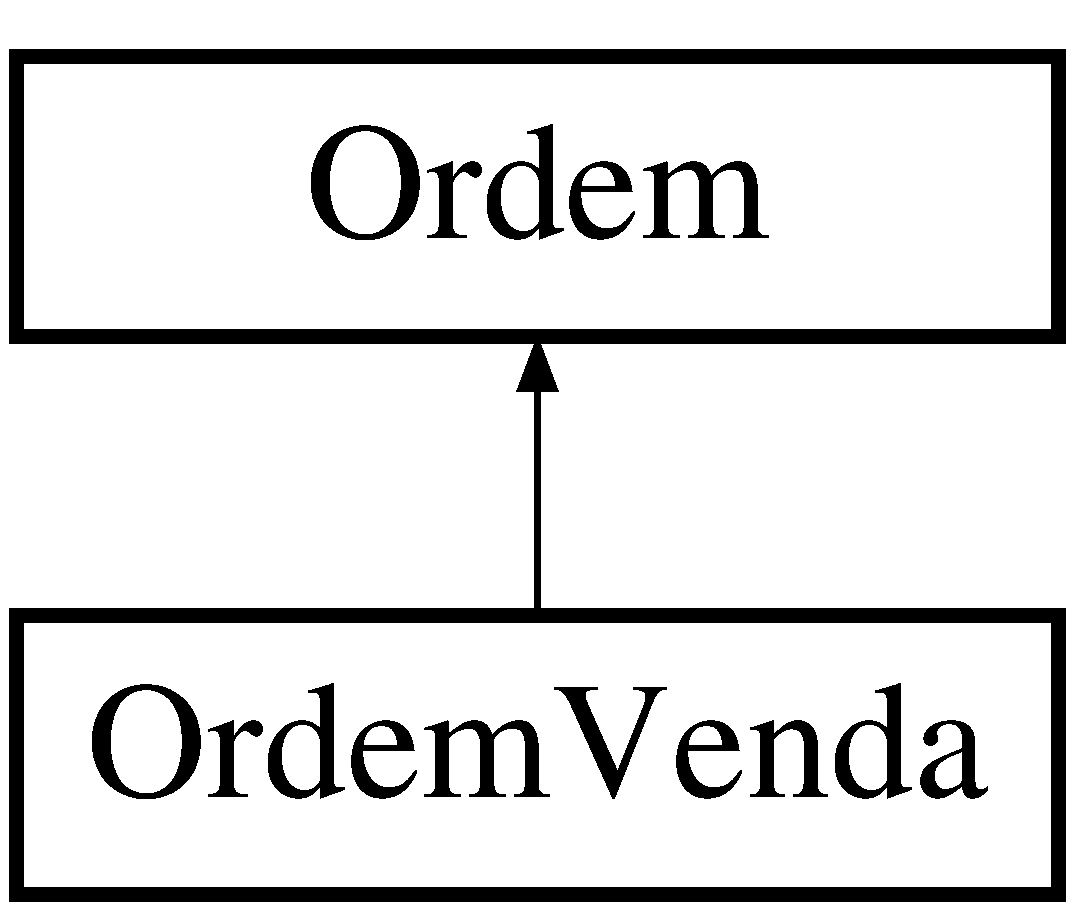
\includegraphics[height=2.000000cm]{class_ordem_venda}
\end{center}
\end{figure}
\subsection*{Public Member Functions}
\begin{DoxyCompactItemize}
\item 
\hyperlink{class_ordem_venda_a90290893a4a714fa7e1b15801a00a452}{Ordem\+Venda} (string \hyperlink{class_ordem_a0773861bd9fb956d5ec62f2ef1de658b}{titulo}, \hyperlink{class_data}{Data} \hyperlink{class_ordem_a9f4dbc2966e98dcbd7e300ae346d8535}{data}, long \hyperlink{class_ordem_af6d06b4250735ae531bdcef5fa332f02}{nif\+\_\+cliente}, int quantidade, float preco\+Min)
\begin{DoxyCompactList}\small\item\em Constructor. \end{DoxyCompactList}\item 
float \hyperlink{class_ordem_venda_a4ebbecbc2fabdeb2f9e6af44c47bd176}{get\+Preco\+Min} () const
\begin{DoxyCompactList}\small\item\em Retorna o preco minimo de venda de cada acao. \end{DoxyCompactList}\item 
void \hyperlink{class_ordem_venda_a5b1ae919558cb5cd7bc892e505abf630}{set\+Preco\+Min} (float preco\+Min)
\begin{DoxyCompactList}\small\item\em Define o preco minimo de venda de cada acao. \end{DoxyCompactList}\item 
int \hyperlink{class_ordem_venda_a0c87b42f245049a1b01f414e508b5692}{get\+Quantidade} () const
\begin{DoxyCompactList}\small\item\em Retorna a quantidade de acoes a vender. \end{DoxyCompactList}\item 
void \hyperlink{class_ordem_venda_a44040292fc692df291cc909d486031de}{set\+Quantidade} (int quantidade)
\begin{DoxyCompactList}\small\item\em Define a quantidade de acoes a vender. \end{DoxyCompactList}\item 
void \hyperlink{class_ordem_venda_a3d6f78188308caac122209e68287e09f}{guardar} (ofstream \&out) const
\begin{DoxyCompactList}\small\item\em Escreve no ficheiro que guarda as informacoes das ordens de venda. \end{DoxyCompactList}\end{DoxyCompactItemize}
\subsection*{Friends}
\begin{DoxyCompactItemize}
\item 
ostream \& \hyperlink{class_ordem_venda_a61ee7a51b949c83f00e5a192bb41e911}{operator$<$$<$} (ostream \&out, const \hyperlink{class_ordem_venda}{Ordem\+Venda} \&ordem)
\begin{DoxyCompactList}\small\item\em Operador para imprimir ordem de venda. \end{DoxyCompactList}\end{DoxyCompactItemize}
\subsection*{Additional Inherited Members}


\subsection{Detailed Description}
Classe que representa uma ordem de venda na bolsa de valores. 

\subsection{Constructor \& Destructor Documentation}
\hypertarget{class_ordem_venda_a90290893a4a714fa7e1b15801a00a452}{}\label{class_ordem_venda_a90290893a4a714fa7e1b15801a00a452} 
\index{Ordem\+Venda@{Ordem\+Venda}!Ordem\+Venda@{Ordem\+Venda}}
\index{Ordem\+Venda@{Ordem\+Venda}!Ordem\+Venda@{Ordem\+Venda}}
\subsubsection{\texorpdfstring{Ordem\+Venda()}{OrdemVenda()}}
{\footnotesize\ttfamily Ordem\+Venda\+::\+Ordem\+Venda (\begin{DoxyParamCaption}\item[{string}]{titulo,  }\item[{\hyperlink{class_data}{Data}}]{data,  }\item[{long}]{nif\+\_\+cliente,  }\item[{int}]{quantidade,  }\item[{float}]{preco\+Min }\end{DoxyParamCaption})}



Constructor. 


\begin{DoxyParams}{Parameters}
{\em titulo} & O titulo da ordem de venda. \\
\hline
{\em data} & A data da ordem de venda. \\
\hline
{\em nif\+\_\+cliente} & O N\+IF do cliente da ordem de venda. \\
\hline
{\em quantidade} & A quantidade de acoes a vender. \\
\hline
{\em preco\+Min} & O preco minimo de venda de cada acao. \\
\hline
\end{DoxyParams}


\subsection{Member Function Documentation}
\hypertarget{class_ordem_venda_a4ebbecbc2fabdeb2f9e6af44c47bd176}{}\label{class_ordem_venda_a4ebbecbc2fabdeb2f9e6af44c47bd176} 
\index{Ordem\+Venda@{Ordem\+Venda}!get\+Preco\+Min@{get\+Preco\+Min}}
\index{get\+Preco\+Min@{get\+Preco\+Min}!Ordem\+Venda@{Ordem\+Venda}}
\subsubsection{\texorpdfstring{get\+Preco\+Min()}{getPrecoMin()}}
{\footnotesize\ttfamily float Ordem\+Venda\+::get\+Preco\+Min (\begin{DoxyParamCaption}{ }\end{DoxyParamCaption}) const\hspace{0.3cm}{\ttfamily [inline]}}



Retorna o preco minimo de venda de cada acao. 

\begin{DoxyReturn}{Returns}
O preco minimo de venda de cada acao. 
\end{DoxyReturn}
\hypertarget{class_ordem_venda_a0c87b42f245049a1b01f414e508b5692}{}\label{class_ordem_venda_a0c87b42f245049a1b01f414e508b5692} 
\index{Ordem\+Venda@{Ordem\+Venda}!get\+Quantidade@{get\+Quantidade}}
\index{get\+Quantidade@{get\+Quantidade}!Ordem\+Venda@{Ordem\+Venda}}
\subsubsection{\texorpdfstring{get\+Quantidade()}{getQuantidade()}}
{\footnotesize\ttfamily int Ordem\+Venda\+::get\+Quantidade (\begin{DoxyParamCaption}{ }\end{DoxyParamCaption}) const\hspace{0.3cm}{\ttfamily [inline]}}



Retorna a quantidade de acoes a vender. 

\begin{DoxyReturn}{Returns}
A quantidade de acoes a vender. 
\end{DoxyReturn}
\hypertarget{class_ordem_venda_a3d6f78188308caac122209e68287e09f}{}\label{class_ordem_venda_a3d6f78188308caac122209e68287e09f} 
\index{Ordem\+Venda@{Ordem\+Venda}!guardar@{guardar}}
\index{guardar@{guardar}!Ordem\+Venda@{Ordem\+Venda}}
\subsubsection{\texorpdfstring{guardar()}{guardar()}}
{\footnotesize\ttfamily void Ordem\+Venda\+::guardar (\begin{DoxyParamCaption}\item[{ofstream \&}]{out }\end{DoxyParamCaption}) const}



Escreve no ficheiro que guarda as informacoes das ordens de venda. 


\begin{DoxyParams}{Parameters}
{\em out} & Ficheiro em que se escreve as informacoes. \\
\hline
\end{DoxyParams}
\hypertarget{class_ordem_venda_a5b1ae919558cb5cd7bc892e505abf630}{}\label{class_ordem_venda_a5b1ae919558cb5cd7bc892e505abf630} 
\index{Ordem\+Venda@{Ordem\+Venda}!set\+Preco\+Min@{set\+Preco\+Min}}
\index{set\+Preco\+Min@{set\+Preco\+Min}!Ordem\+Venda@{Ordem\+Venda}}
\subsubsection{\texorpdfstring{set\+Preco\+Min()}{setPrecoMin()}}
{\footnotesize\ttfamily void Ordem\+Venda\+::set\+Preco\+Min (\begin{DoxyParamCaption}\item[{float}]{preco\+Min }\end{DoxyParamCaption})\hspace{0.3cm}{\ttfamily [inline]}}



Define o preco minimo de venda de cada acao. 


\begin{DoxyParams}{Parameters}
{\em preco\+Min} & O preco minimo de venda de cada acao. \\
\hline
\end{DoxyParams}
\hypertarget{class_ordem_venda_a44040292fc692df291cc909d486031de}{}\label{class_ordem_venda_a44040292fc692df291cc909d486031de} 
\index{Ordem\+Venda@{Ordem\+Venda}!set\+Quantidade@{set\+Quantidade}}
\index{set\+Quantidade@{set\+Quantidade}!Ordem\+Venda@{Ordem\+Venda}}
\subsubsection{\texorpdfstring{set\+Quantidade()}{setQuantidade()}}
{\footnotesize\ttfamily void Ordem\+Venda\+::set\+Quantidade (\begin{DoxyParamCaption}\item[{int}]{quantidade }\end{DoxyParamCaption})\hspace{0.3cm}{\ttfamily [inline]}}



Define a quantidade de acoes a vender. 


\begin{DoxyParams}{Parameters}
{\em quantidade} & A quantidade de acoes a vender. \\
\hline
\end{DoxyParams}


\subsection{Friends And Related Function Documentation}
\hypertarget{class_ordem_venda_a61ee7a51b949c83f00e5a192bb41e911}{}\label{class_ordem_venda_a61ee7a51b949c83f00e5a192bb41e911} 
\index{Ordem\+Venda@{Ordem\+Venda}!operator$<$$<$@{operator$<$$<$}}
\index{operator$<$$<$@{operator$<$$<$}!Ordem\+Venda@{Ordem\+Venda}}
\subsubsection{\texorpdfstring{operator$<$$<$}{operator<<}}
{\footnotesize\ttfamily ostream \& operator$<$$<$ (\begin{DoxyParamCaption}\item[{ostream \&}]{out,  }\item[{const \hyperlink{class_ordem_venda}{Ordem\+Venda} \&}]{ordem }\end{DoxyParamCaption})\hspace{0.3cm}{\ttfamily [friend]}}



Operador para imprimir ordem de venda. 


\begin{DoxyParams}[1]{Parameters}
\mbox{\tt in,out}  & {\em out} & Onde imprime a ordem de venda. \\
\hline
 & {\em ordem} & A ordem de venda a imprimir. \\
\hline
\end{DoxyParams}


The documentation for this class was generated from the following files\+:\begin{DoxyCompactItemize}
\item 
\hyperlink{_ordem_venda_8h}{Ordem\+Venda.\+h}\item 
\hyperlink{_ordem_venda_8cpp}{Ordem\+Venda.\+cpp}\end{DoxyCompactItemize}

\hypertarget{class_transacao}{}\section{Transacao Class Reference}
\label{class_transacao}\index{Transacao@{Transacao}}


Classe que representa uma transacao na bolsa de valores.  




{\ttfamily \#include $<$Transacao.\+h$>$}

\subsection*{Public Member Functions}
\begin{DoxyCompactItemize}
\item 
\hyperlink{class_transacao_a85413a667a5e4e7632c7926900d3d517}{Transacao} (string titulo, float preco\+\_\+acao, int num\+\_\+acoes, \hyperlink{class_data}{Data} data, long cliente\+\_\+v, long cliente\+\_\+c)
\begin{DoxyCompactList}\small\item\em Constructor. \end{DoxyCompactList}\item 
\hyperlink{class_transacao_adad7dd2c36a20c16e0ac40e3a5822650}{Transacao} (ifstream \&in)
\begin{DoxyCompactList}\small\item\em Constructor que le uma linha de um ficheiro de texto. \end{DoxyCompactList}\item 
bool \hyperlink{class_transacao_a99deb0eadbb36741646610299c2fecad}{operator$<$} (const \hyperlink{class_transacao}{Transacao} \&tr) const
\begin{DoxyCompactList}\small\item\em Compara as transacoes por data. \end{DoxyCompactList}\item 
string \hyperlink{class_transacao_af48d21e7643548e9b8ff9ee9d1cd39c8}{get\+Titulo} ()
\begin{DoxyCompactList}\small\item\em Retorna o titulo da acao da transacao. \end{DoxyCompactList}\item 
float \hyperlink{class_transacao_a04806fca6de35ac9f57044c2bd2c39b3}{get\+Preco\+\_\+acao} ()
\begin{DoxyCompactList}\small\item\em Retorna o preco por acao da transacao. \end{DoxyCompactList}\item 
int \hyperlink{class_transacao_af52a47c91fe23258ddd212a78f044297}{get\+Num\+\_\+acoes} ()
\begin{DoxyCompactList}\small\item\em Retorna o numero de acoes. \end{DoxyCompactList}\item 
\hyperlink{class_data}{Data} \hyperlink{class_transacao_a94162db1ef8a17eee755c3a3c1d7744b}{get\+Data} ()
\begin{DoxyCompactList}\small\item\em Retorna a data da transacao. \end{DoxyCompactList}\item 
long \hyperlink{class_transacao_a67521a6dea9a82ca2d7d3821a10a6e0d}{get\+Cliente\+\_\+v} ()
\begin{DoxyCompactList}\small\item\em Retorna o N\+IF do cliente que vende as acoes. \end{DoxyCompactList}\item 
long \hyperlink{class_transacao_ad896abaa081d1407b69f8bd9a60b107c}{get\+Cliente\+\_\+c} ()
\begin{DoxyCompactList}\small\item\em Retorna o N\+IF do cliente que compra as acoes. \end{DoxyCompactList}\item 
void \hyperlink{class_transacao_aa4b2e7563ee4cb46bea35ea5b8d5f96a}{guardar} (ofstream \&out) const
\begin{DoxyCompactList}\small\item\em Escreve num ficheiro que guarda as informacoes das transacoes. \end{DoxyCompactList}\end{DoxyCompactItemize}
\subsection*{Friends}
\begin{DoxyCompactItemize}
\item 
ostream \& \hyperlink{class_transacao_a1b84445ef2674a7af30a1d313844766c}{operator$<$$<$} (ostream \&out, const \hyperlink{class_transacao}{Transacao} \&transacao)
\begin{DoxyCompactList}\small\item\em Operador para imprimir uma transacao. \end{DoxyCompactList}\end{DoxyCompactItemize}


\subsection{Detailed Description}
Classe que representa uma transacao na bolsa de valores. 

\subsection{Constructor \& Destructor Documentation}
\hypertarget{class_transacao_a85413a667a5e4e7632c7926900d3d517}{}\label{class_transacao_a85413a667a5e4e7632c7926900d3d517} 
\index{Transacao@{Transacao}!Transacao@{Transacao}}
\index{Transacao@{Transacao}!Transacao@{Transacao}}
\subsubsection{\texorpdfstring{Transacao()}{Transacao()}\hspace{0.1cm}{\footnotesize\ttfamily [1/2]}}
{\footnotesize\ttfamily Transacao\+::\+Transacao (\begin{DoxyParamCaption}\item[{string}]{titulo,  }\item[{float}]{preco\+\_\+acao,  }\item[{int}]{num\+\_\+acoes,  }\item[{\hyperlink{class_data}{Data}}]{data,  }\item[{long}]{cliente\+\_\+v,  }\item[{long}]{cliente\+\_\+c }\end{DoxyParamCaption})}



Constructor. 


\begin{DoxyParams}{Parameters}
{\em titulo} & O titulo da acao da transacao. \\
\hline
{\em preco\+\_\+acao} & O preso da acao. \\
\hline
{\em num\+\_\+acoes} & Numero de acoes da transacao. \\
\hline
{\em data} & A data da transacao. \\
\hline
{\em cliente\+\_\+v} & O N\+IF do cliente que vende as acoes. \\
\hline
{\em cliente\+\_\+c} & O N\+IF do cliente que compra as acoes. \\
\hline
\end{DoxyParams}
\hypertarget{class_transacao_adad7dd2c36a20c16e0ac40e3a5822650}{}\label{class_transacao_adad7dd2c36a20c16e0ac40e3a5822650} 
\index{Transacao@{Transacao}!Transacao@{Transacao}}
\index{Transacao@{Transacao}!Transacao@{Transacao}}
\subsubsection{\texorpdfstring{Transacao()}{Transacao()}\hspace{0.1cm}{\footnotesize\ttfamily [2/2]}}
{\footnotesize\ttfamily Transacao\+::\+Transacao (\begin{DoxyParamCaption}\item[{ifstream \&}]{in }\end{DoxyParamCaption})}



Constructor que le uma linha de um ficheiro de texto. 


\begin{DoxyParams}{Parameters}
{\em in} & Ficheiro de texto. \\
\hline
\end{DoxyParams}


\subsection{Member Function Documentation}
\hypertarget{class_transacao_ad896abaa081d1407b69f8bd9a60b107c}{}\label{class_transacao_ad896abaa081d1407b69f8bd9a60b107c} 
\index{Transacao@{Transacao}!get\+Cliente\+\_\+c@{get\+Cliente\+\_\+c}}
\index{get\+Cliente\+\_\+c@{get\+Cliente\+\_\+c}!Transacao@{Transacao}}
\subsubsection{\texorpdfstring{get\+Cliente\+\_\+c()}{getCliente\_c()}}
{\footnotesize\ttfamily long Transacao\+::get\+Cliente\+\_\+c (\begin{DoxyParamCaption}{ }\end{DoxyParamCaption})}



Retorna o N\+IF do cliente que compra as acoes. 

\begin{DoxyReturn}{Returns}
O N\+IF do cliente que vende as acoes. 
\end{DoxyReturn}
\hypertarget{class_transacao_a67521a6dea9a82ca2d7d3821a10a6e0d}{}\label{class_transacao_a67521a6dea9a82ca2d7d3821a10a6e0d} 
\index{Transacao@{Transacao}!get\+Cliente\+\_\+v@{get\+Cliente\+\_\+v}}
\index{get\+Cliente\+\_\+v@{get\+Cliente\+\_\+v}!Transacao@{Transacao}}
\subsubsection{\texorpdfstring{get\+Cliente\+\_\+v()}{getCliente\_v()}}
{\footnotesize\ttfamily long Transacao\+::get\+Cliente\+\_\+v (\begin{DoxyParamCaption}{ }\end{DoxyParamCaption})}



Retorna o N\+IF do cliente que vende as acoes. 

\begin{DoxyReturn}{Returns}
O N\+IF do cliente que vende as acoes. 
\end{DoxyReturn}
\hypertarget{class_transacao_a94162db1ef8a17eee755c3a3c1d7744b}{}\label{class_transacao_a94162db1ef8a17eee755c3a3c1d7744b} 
\index{Transacao@{Transacao}!get\+Data@{get\+Data}}
\index{get\+Data@{get\+Data}!Transacao@{Transacao}}
\subsubsection{\texorpdfstring{get\+Data()}{getData()}}
{\footnotesize\ttfamily \hyperlink{class_data}{Data} Transacao\+::get\+Data (\begin{DoxyParamCaption}{ }\end{DoxyParamCaption})}



Retorna a data da transacao. 

\begin{DoxyReturn}{Returns}
The data. 
\end{DoxyReturn}
\hypertarget{class_transacao_af52a47c91fe23258ddd212a78f044297}{}\label{class_transacao_af52a47c91fe23258ddd212a78f044297} 
\index{Transacao@{Transacao}!get\+Num\+\_\+acoes@{get\+Num\+\_\+acoes}}
\index{get\+Num\+\_\+acoes@{get\+Num\+\_\+acoes}!Transacao@{Transacao}}
\subsubsection{\texorpdfstring{get\+Num\+\_\+acoes()}{getNum\_acoes()}}
{\footnotesize\ttfamily int Transacao\+::get\+Num\+\_\+acoes (\begin{DoxyParamCaption}{ }\end{DoxyParamCaption})}



Retorna o numero de acoes. 

\begin{DoxyReturn}{Returns}
O numero de acoes. 
\end{DoxyReturn}
\hypertarget{class_transacao_a04806fca6de35ac9f57044c2bd2c39b3}{}\label{class_transacao_a04806fca6de35ac9f57044c2bd2c39b3} 
\index{Transacao@{Transacao}!get\+Preco\+\_\+acao@{get\+Preco\+\_\+acao}}
\index{get\+Preco\+\_\+acao@{get\+Preco\+\_\+acao}!Transacao@{Transacao}}
\subsubsection{\texorpdfstring{get\+Preco\+\_\+acao()}{getPreco\_acao()}}
{\footnotesize\ttfamily float Transacao\+::get\+Preco\+\_\+acao (\begin{DoxyParamCaption}{ }\end{DoxyParamCaption})}



Retorna o preco por acao da transacao. 

\begin{DoxyReturn}{Returns}
O preco por acao da transacao. 
\end{DoxyReturn}
\hypertarget{class_transacao_af48d21e7643548e9b8ff9ee9d1cd39c8}{}\label{class_transacao_af48d21e7643548e9b8ff9ee9d1cd39c8} 
\index{Transacao@{Transacao}!get\+Titulo@{get\+Titulo}}
\index{get\+Titulo@{get\+Titulo}!Transacao@{Transacao}}
\subsubsection{\texorpdfstring{get\+Titulo()}{getTitulo()}}
{\footnotesize\ttfamily string Transacao\+::get\+Titulo (\begin{DoxyParamCaption}{ }\end{DoxyParamCaption})}



Retorna o titulo da acao da transacao. 

\begin{DoxyReturn}{Returns}
O titulo da acao da transacao. 
\end{DoxyReturn}
\hypertarget{class_transacao_aa4b2e7563ee4cb46bea35ea5b8d5f96a}{}\label{class_transacao_aa4b2e7563ee4cb46bea35ea5b8d5f96a} 
\index{Transacao@{Transacao}!guardar@{guardar}}
\index{guardar@{guardar}!Transacao@{Transacao}}
\subsubsection{\texorpdfstring{guardar()}{guardar()}}
{\footnotesize\ttfamily void Transacao\+::guardar (\begin{DoxyParamCaption}\item[{ofstream \&}]{out }\end{DoxyParamCaption}) const}



Escreve num ficheiro que guarda as informacoes das transacoes. 


\begin{DoxyParams}{Parameters}
{\em out} & Ficheiro em que se escreve as informacoes. \\
\hline
\end{DoxyParams}
\hypertarget{class_transacao_a99deb0eadbb36741646610299c2fecad}{}\label{class_transacao_a99deb0eadbb36741646610299c2fecad} 
\index{Transacao@{Transacao}!operator$<$@{operator$<$}}
\index{operator$<$@{operator$<$}!Transacao@{Transacao}}
\subsubsection{\texorpdfstring{operator$<$()}{operator<()}}
{\footnotesize\ttfamily bool Transacao\+::operator$<$ (\begin{DoxyParamCaption}\item[{const \hyperlink{class_transacao}{Transacao} \&}]{tr }\end{DoxyParamCaption}) const}



Compara as transacoes por data. 


\begin{DoxyParams}{Parameters}
{\em tr} & Segunda transacao a comparar.\\
\hline
\end{DoxyParams}
\begin{DoxyReturn}{Returns}
Verdade se a data da primeira transacao for menor que da segunda. 
\end{DoxyReturn}


\subsection{Friends And Related Function Documentation}
\hypertarget{class_transacao_a1b84445ef2674a7af30a1d313844766c}{}\label{class_transacao_a1b84445ef2674a7af30a1d313844766c} 
\index{Transacao@{Transacao}!operator$<$$<$@{operator$<$$<$}}
\index{operator$<$$<$@{operator$<$$<$}!Transacao@{Transacao}}
\subsubsection{\texorpdfstring{operator$<$$<$}{operator<<}}
{\footnotesize\ttfamily ostream \& operator$<$$<$ (\begin{DoxyParamCaption}\item[{ostream \&}]{out,  }\item[{const \hyperlink{class_transacao}{Transacao} \&}]{transacao }\end{DoxyParamCaption})\hspace{0.3cm}{\ttfamily [friend]}}



Operador para imprimir uma transacao. 


\begin{DoxyParams}{Parameters}
{\em out} & Onde imprime a transacao. \\
\hline
{\em transacao} & A transacao a imprimir. \\
\hline
\end{DoxyParams}


The documentation for this class was generated from the following files\+:\begin{DoxyCompactItemize}
\item 
\hyperlink{_transacao_8h}{Transacao.\+h}\item 
\hyperlink{_transacao_8cpp}{Transacao.\+cpp}\end{DoxyCompactItemize}

\chapter{File Documentation}
\hypertarget{_bolsa_8cpp}{}\section{Bolsa.\+cpp File Reference}
\label{_bolsa_8cpp}\index{Bolsa.\+cpp@{Bolsa.\+cpp}}
{\ttfamily \#include \char`\"{}Bolsa.\+h\char`\"{}}\newline

\hypertarget{_bolsa_8h}{}\section{Bolsa.\+h File Reference}
\label{_bolsa_8h}\index{Bolsa.\+h@{Bolsa.\+h}}
{\ttfamily \#include $<$iostream$>$}\newline
{\ttfamily \#include $<$vector$>$}\newline
{\ttfamily \#include $<$fstream$>$}\newline
{\ttfamily \#include $<$iomanip$>$}\newline
{\ttfamily \#include \char`\"{}Ordem\+Venda.\+h\char`\"{}}\newline
{\ttfamily \#include \char`\"{}Ordem\+Compra.\+h\char`\"{}}\newline
{\ttfamily \#include \char`\"{}Cliente.\+h\char`\"{}}\newline
{\ttfamily \#include \char`\"{}Utils.\+h\char`\"{}}\newline
{\ttfamily \#include \char`\"{}Transacao.\+h\char`\"{}}\newline
{\ttfamily \#include \char`\"{}insertion\+Sort.\+h\char`\"{}}\newline
\subsection*{Classes}
\begin{DoxyCompactItemize}
\item 
class \hyperlink{class_bolsa}{Bolsa}
\begin{DoxyCompactList}\small\item\em Classe que guarda os clientes, ordens de compra e venda, e transacoes da bolsa e as funcoes para manipulacao da mesma. \end{DoxyCompactList}\end{DoxyCompactItemize}

\hypertarget{_cliente_8cpp}{}\section{Cliente.\+cpp File Reference}
\label{_cliente_8cpp}\index{Cliente.\+cpp@{Cliente.\+cpp}}
{\ttfamily \#include \char`\"{}Cliente.\+h\char`\"{}}\newline

\hypertarget{_cliente_8h}{}\section{Cliente.\+h File Reference}
\label{_cliente_8h}\index{Cliente.\+h@{Cliente.\+h}}
{\ttfamily \#include $<$string$>$}\newline
{\ttfamily \#include $<$iostream$>$}\newline
{\ttfamily \#include $<$fstream$>$}\newline
\subsection*{Classes}
\begin{DoxyCompactItemize}
\item 
class \hyperlink{class_cliente}{Cliente}
\begin{DoxyCompactList}\small\item\em Classe que guarda o nome e o nif do cliente e as funcoes para manipulacao da mesma. \end{DoxyCompactList}\end{DoxyCompactItemize}

\hypertarget{_data_8cpp}{}\section{Data.\+cpp File Reference}
\label{_data_8cpp}\index{Data.\+cpp@{Data.\+cpp}}
{\ttfamily \#include \char`\"{}Data.\+h\char`\"{}}\newline
\subsection*{Functions}
\begin{DoxyCompactItemize}
\item 
ostream \& \hyperlink{_data_8cpp_a90bb051fbc9d2b01d7a4936fc42cd7a9}{operator$<$$<$} (ostream \&os, const \hyperlink{class_data}{Data} \&d)
\end{DoxyCompactItemize}


\subsection{Function Documentation}
\hypertarget{_data_8cpp_a90bb051fbc9d2b01d7a4936fc42cd7a9}{}\label{_data_8cpp_a90bb051fbc9d2b01d7a4936fc42cd7a9} 
\index{Data.\+cpp@{Data.\+cpp}!operator$<$$<$@{operator$<$$<$}}
\index{operator$<$$<$@{operator$<$$<$}!Data.\+cpp@{Data.\+cpp}}
\subsubsection{\texorpdfstring{operator$<$$<$()}{operator<<()}}
{\footnotesize\ttfamily ostream\& operator$<$$<$ (\begin{DoxyParamCaption}\item[{ostream \&}]{os,  }\item[{const \hyperlink{class_data}{Data} \&}]{d }\end{DoxyParamCaption})}


\hypertarget{_data_8h}{}\section{Data.\+h File Reference}
\label{_data_8h}\index{Data.\+h@{Data.\+h}}
{\ttfamily \#include $<$iostream$>$}\newline
{\ttfamily \#include $<$sstream$>$}\newline
{\ttfamily \#include $<$string$>$}\newline
{\ttfamily \#include $<$iomanip$>$}\newline
\subsection*{Classes}
\begin{DoxyCompactItemize}
\item 
class \hyperlink{class_data}{Data}
\begin{DoxyCompactList}\small\item\em Classe que guarda o dia, mes e ano e as funcoes para manipulacao da mesma. \end{DoxyCompactList}\end{DoxyCompactItemize}

\hypertarget{_excecoes_8cpp}{}\section{Excecoes.\+cpp File Reference}
\label{_excecoes_8cpp}\index{Excecoes.\+cpp@{Excecoes.\+cpp}}
{\ttfamily \#include \char`\"{}Excecoes.\+h\char`\"{}}\newline
\subsection*{Functions}
\begin{DoxyCompactItemize}
\item 
ostream \& \hyperlink{_excecoes_8cpp_aadb54278cd2995f4fbae46df928e82bf}{operator$<$$<$} (ostream \&out, const \hyperlink{class_ficheiro_inexistente}{Ficheiro\+Inexistente} \&fich\+\_\+inex)
\item 
ostream \& \hyperlink{_excecoes_8cpp_a1b3204d4e9fc715ae1f42b8ef53a6db6}{operator$<$$<$} (ostream \&out, const \hyperlink{class_ficheiro_invalido}{Ficheiro\+Invalido} \&fich\+\_\+inva)
\end{DoxyCompactItemize}


\subsection{Function Documentation}
\hypertarget{_excecoes_8cpp_aadb54278cd2995f4fbae46df928e82bf}{}\label{_excecoes_8cpp_aadb54278cd2995f4fbae46df928e82bf} 
\index{Excecoes.\+cpp@{Excecoes.\+cpp}!operator$<$$<$@{operator$<$$<$}}
\index{operator$<$$<$@{operator$<$$<$}!Excecoes.\+cpp@{Excecoes.\+cpp}}
\subsubsection{\texorpdfstring{operator$<$$<$()}{operator<<()}\hspace{0.1cm}{\footnotesize\ttfamily [1/2]}}
{\footnotesize\ttfamily ostream\& operator$<$$<$ (\begin{DoxyParamCaption}\item[{ostream \&}]{out,  }\item[{const \hyperlink{class_ficheiro_inexistente}{Ficheiro\+Inexistente} \&}]{fich\+\_\+inex }\end{DoxyParamCaption})}

\hypertarget{_excecoes_8cpp_a1b3204d4e9fc715ae1f42b8ef53a6db6}{}\label{_excecoes_8cpp_a1b3204d4e9fc715ae1f42b8ef53a6db6} 
\index{Excecoes.\+cpp@{Excecoes.\+cpp}!operator$<$$<$@{operator$<$$<$}}
\index{operator$<$$<$@{operator$<$$<$}!Excecoes.\+cpp@{Excecoes.\+cpp}}
\subsubsection{\texorpdfstring{operator$<$$<$()}{operator<<()}\hspace{0.1cm}{\footnotesize\ttfamily [2/2]}}
{\footnotesize\ttfamily ostream\& operator$<$$<$ (\begin{DoxyParamCaption}\item[{ostream \&}]{out,  }\item[{const \hyperlink{class_ficheiro_invalido}{Ficheiro\+Invalido} \&}]{fich\+\_\+inva }\end{DoxyParamCaption})}


\hypertarget{_excecoes_8h}{}\section{Excecoes.\+h File Reference}
\label{_excecoes_8h}\index{Excecoes.\+h@{Excecoes.\+h}}
{\ttfamily \#include $<$string$>$}\newline
\subsection*{Classes}
\begin{DoxyCompactItemize}
\item 
class \hyperlink{class_ficheiro_inexistente}{Ficheiro\+Inexistente}
\begin{DoxyCompactList}\small\item\em Excecao que e lancada quando se tenta abrir um ficheiro inexistente. \end{DoxyCompactList}\item 
class \hyperlink{class_ficheiro_invalido}{Ficheiro\+Invalido}
\begin{DoxyCompactList}\small\item\em Excecao que e lancada quando se abre um ficheiro invalido. \end{DoxyCompactList}\end{DoxyCompactItemize}

\hypertarget{insertion_sort_8h}{}\section{insertion\+Sort.\+h File Reference}
\label{insertion_sort_8h}\index{insertion\+Sort.\+h@{insertion\+Sort.\+h}}
{\ttfamily \#include $<$vector$>$}\newline
\subsection*{Functions}
\begin{DoxyCompactItemize}
\item 
{\footnotesize template$<$class Comparable $>$ }\\void \hyperlink{insertion_sort_8h_a9bec216ad15dc4199bf30ade4400bc1a}{insertion\+Sort} (vector$<$ Comparable $>$ \&v)
\begin{DoxyCompactList}\small\item\em Ordenacao de um vetor pelo m�todo insertion Sort. \end{DoxyCompactList}\end{DoxyCompactItemize}


\subsection{Function Documentation}
\hypertarget{insertion_sort_8h_a9bec216ad15dc4199bf30ade4400bc1a}{}\label{insertion_sort_8h_a9bec216ad15dc4199bf30ade4400bc1a} 
\index{insertion\+Sort.\+h@{insertion\+Sort.\+h}!insertion\+Sort@{insertion\+Sort}}
\index{insertion\+Sort@{insertion\+Sort}!insertion\+Sort.\+h@{insertion\+Sort.\+h}}
\subsubsection{\texorpdfstring{insertion\+Sort()}{insertionSort()}}
{\footnotesize\ttfamily template$<$class Comparable $>$ \\
template$<$ class Comparable $>$ void insertion\+Sort (\begin{DoxyParamCaption}\item[{vector$<$ Comparable $>$ \&}]{v }\end{DoxyParamCaption})}



Ordenacao de um vetor pelo m�todo insertion Sort. 


\begin{DoxyParams}{Parameters}
{\em v} & Vetor a ordenar. \\
\hline
\end{DoxyParams}

\hypertarget{main_8cpp}{}\section{main.\+cpp File Reference}
\label{main_8cpp}\index{main.\+cpp@{main.\+cpp}}
{\ttfamily \#include \char`\"{}Bolsa.\+h\char`\"{}}\newline
{\ttfamily \#include \char`\"{}Data.\+h\char`\"{}}\newline
{\ttfamily \#include \char`\"{}Menus.\+h\char`\"{}}\newline
{\ttfamily \#include \char`\"{}Utils.\+h\char`\"{}}\newline
{\ttfamily \#include $<$iostream$>$}\newline
{\ttfamily \#include $<$fstream$>$}\newline
{\ttfamily \#include $<$string$>$}\newline
{\ttfamily \#include $<$vector$>$}\newline
\subsection*{Functions}
\begin{DoxyCompactItemize}
\item 
int \hyperlink{main_8cpp_ae66f6b31b5ad750f1fe042a706a4e3d4}{main} ()
\end{DoxyCompactItemize}
\subsection*{Variables}
\begin{DoxyCompactItemize}
\item 
string \hyperlink{main_8cpp_a1335b18f135ed58c716b3ddcecdc8cce}{fich\+Clientes}
\item 
string \hyperlink{main_8cpp_a66ff7fedd13a1b40664042a086ca0f27}{fich\+Transacoes}
\item 
string \hyperlink{main_8cpp_ad22902af7efe6d185550055b7caa5cbb}{fich\+Ordens\+Venda}
\item 
string \hyperlink{main_8cpp_a06ef2704898a1a2529cd2d724426f9c0}{fich\+Ordens\+Compra}
\begin{DoxyCompactList}\small\item\em Guarda os nomes dos ficheiros com os dados externamente para serem usados em varias fun�oes. \end{DoxyCompactList}\end{DoxyCompactItemize}


\subsection{Function Documentation}
\hypertarget{main_8cpp_ae66f6b31b5ad750f1fe042a706a4e3d4}{}\label{main_8cpp_ae66f6b31b5ad750f1fe042a706a4e3d4} 
\index{main.\+cpp@{main.\+cpp}!main@{main}}
\index{main@{main}!main.\+cpp@{main.\+cpp}}
\subsubsection{\texorpdfstring{main()}{main()}}
{\footnotesize\ttfamily int main (\begin{DoxyParamCaption}{ }\end{DoxyParamCaption})}



\subsection{Variable Documentation}
\hypertarget{main_8cpp_a1335b18f135ed58c716b3ddcecdc8cce}{}\label{main_8cpp_a1335b18f135ed58c716b3ddcecdc8cce} 
\index{main.\+cpp@{main.\+cpp}!fich\+Clientes@{fich\+Clientes}}
\index{fich\+Clientes@{fich\+Clientes}!main.\+cpp@{main.\+cpp}}
\subsubsection{\texorpdfstring{fich\+Clientes}{fichClientes}}
{\footnotesize\ttfamily string fich\+Clientes}

\hypertarget{main_8cpp_a06ef2704898a1a2529cd2d724426f9c0}{}\label{main_8cpp_a06ef2704898a1a2529cd2d724426f9c0} 
\index{main.\+cpp@{main.\+cpp}!fich\+Ordens\+Compra@{fich\+Ordens\+Compra}}
\index{fich\+Ordens\+Compra@{fich\+Ordens\+Compra}!main.\+cpp@{main.\+cpp}}
\subsubsection{\texorpdfstring{fich\+Ordens\+Compra}{fichOrdensCompra}}
{\footnotesize\ttfamily string \hyperlink{_utils_8h_a1335b18f135ed58c716b3ddcecdc8cce}{fich\+Clientes} \hyperlink{_utils_8h_a66ff7fedd13a1b40664042a086ca0f27}{fich\+Transacoes} \hyperlink{_utils_8h_ad22902af7efe6d185550055b7caa5cbb}{fich\+Ordens\+Venda} fich\+Ordens\+Compra}



Guarda os nomes dos ficheiros com os dados externamente para serem usados em varias fun�oes. 

\hypertarget{main_8cpp_ad22902af7efe6d185550055b7caa5cbb}{}\label{main_8cpp_ad22902af7efe6d185550055b7caa5cbb} 
\index{main.\+cpp@{main.\+cpp}!fich\+Ordens\+Venda@{fich\+Ordens\+Venda}}
\index{fich\+Ordens\+Venda@{fich\+Ordens\+Venda}!main.\+cpp@{main.\+cpp}}
\subsubsection{\texorpdfstring{fich\+Ordens\+Venda}{fichOrdensVenda}}
{\footnotesize\ttfamily string fich\+Ordens\+Venda}

\hypertarget{main_8cpp_a66ff7fedd13a1b40664042a086ca0f27}{}\label{main_8cpp_a66ff7fedd13a1b40664042a086ca0f27} 
\index{main.\+cpp@{main.\+cpp}!fich\+Transacoes@{fich\+Transacoes}}
\index{fich\+Transacoes@{fich\+Transacoes}!main.\+cpp@{main.\+cpp}}
\subsubsection{\texorpdfstring{fich\+Transacoes}{fichTransacoes}}
{\footnotesize\ttfamily string fich\+Transacoes}


\hypertarget{_menus_8cpp}{}\section{Menus.\+cpp File Reference}
\label{_menus_8cpp}\index{Menus.\+cpp@{Menus.\+cpp}}
{\ttfamily \#include \char`\"{}Menus.\+h\char`\"{}}\newline
\subsection*{Functions}
\begin{DoxyCompactItemize}
\item 
int \hyperlink{_menus_8cpp_a1ea89981ed52e2e57eca0d22a00817f2}{verfica\+\_\+fich} (string \&fich\+\_\+veri, string tipo\+\_\+fich)
\begin{DoxyCompactList}\small\item\em Verfica se fich\+\_\+veri existe e se e valido. \end{DoxyCompactList}\item 
int \hyperlink{_menus_8cpp_a978c7557eca55fb477d0e41bf13b2da9}{info\+Inicial} (string \&\hyperlink{_utils_8h_a1335b18f135ed58c716b3ddcecdc8cce}{fich\+Clientes}, string \&\hyperlink{_utils_8h_a66ff7fedd13a1b40664042a086ca0f27}{fich\+Transacoes}, string \&\hyperlink{_utils_8h_ad22902af7efe6d185550055b7caa5cbb}{fich\+Ordens\+Venda}, string \&\hyperlink{_utils_8h_acaee3ba642d3be244820a97e5eb5b7f7}{fich\+Ordens\+Compra})
\begin{DoxyCompactList}\small\item\em Verifica os 4 ficheiros de dados com a funcao verifica\+\_\+fich. \end{DoxyCompactList}\item 
unsigned short int \hyperlink{_menus_8cpp_a583f75692d29bdfc501b6679b6d2f426}{menu\+Inicial} ()
\item 
void \hyperlink{_menus_8cpp_a128e37d4671a56ab0fcd512eb2454f64}{opcoes\+Iniciais} (\hyperlink{class_bolsa}{Bolsa} \&bolsa\+\_\+de\+\_\+valores)
\begin{DoxyCompactList}\small\item\em Le a opcao do utilizadoe do menu inicial. \end{DoxyCompactList}\item 
void \hyperlink{_menus_8cpp_af1397c4e7e9d57be0c3bac54ff27188e}{menu\+Transacoes} (\hyperlink{class_bolsa}{Bolsa} \&bolsa\+\_\+de\+\_\+valores)
\begin{DoxyCompactList}\small\item\em Apresenta o menu com as varias opcoes para listar as transacoes. \end{DoxyCompactList}\end{DoxyCompactItemize}


\subsection{Function Documentation}
\hypertarget{_menus_8cpp_a978c7557eca55fb477d0e41bf13b2da9}{}\label{_menus_8cpp_a978c7557eca55fb477d0e41bf13b2da9} 
\index{Menus.\+cpp@{Menus.\+cpp}!info\+Inicial@{info\+Inicial}}
\index{info\+Inicial@{info\+Inicial}!Menus.\+cpp@{Menus.\+cpp}}
\subsubsection{\texorpdfstring{info\+Inicial()}{infoInicial()}}
{\footnotesize\ttfamily int info\+Inicial (\begin{DoxyParamCaption}\item[{string \&}]{fich\+Clientes,  }\item[{string \&}]{fich\+Transacoes,  }\item[{string \&}]{fich\+Ordens\+Venda,  }\item[{string \&}]{fich\+Ordens\+Compra }\end{DoxyParamCaption})}



Verifica os 4 ficheiros de dados com a funcao verifica\+\_\+fich. 


\begin{DoxyParams}{Parameters}
{\em fich\+Clientes} & O ficheiro com as informacoes dos clientes. \\
\hline
{\em fich\+Transacoes} & O ficheiro com as informacoes das transacoes. \\
\hline
{\em fich\+Ordens\+Venda} & O ficheiro com as informacoes das ordens venda. \\
\hline
{\em fich\+Ordens\+Compra} & O ficheiro com as informacoes das ordens compra.\\
\hline
\end{DoxyParams}
\begin{DoxyReturn}{Returns}
1 se um dos 4 ficheiros nao for valido e 0 se todos forem validos. 
\end{DoxyReturn}
\hypertarget{_menus_8cpp_a583f75692d29bdfc501b6679b6d2f426}{}\label{_menus_8cpp_a583f75692d29bdfc501b6679b6d2f426} 
\index{Menus.\+cpp@{Menus.\+cpp}!menu\+Inicial@{menu\+Inicial}}
\index{menu\+Inicial@{menu\+Inicial}!Menus.\+cpp@{Menus.\+cpp}}
\subsubsection{\texorpdfstring{menu\+Inicial()}{menuInicial()}}
{\footnotesize\ttfamily unsigned short int menu\+Inicial (\begin{DoxyParamCaption}{ }\end{DoxyParamCaption})}

\hypertarget{_menus_8cpp_af1397c4e7e9d57be0c3bac54ff27188e}{}\label{_menus_8cpp_af1397c4e7e9d57be0c3bac54ff27188e} 
\index{Menus.\+cpp@{Menus.\+cpp}!menu\+Transacoes@{menu\+Transacoes}}
\index{menu\+Transacoes@{menu\+Transacoes}!Menus.\+cpp@{Menus.\+cpp}}
\subsubsection{\texorpdfstring{menu\+Transacoes()}{menuTransacoes()}}
{\footnotesize\ttfamily void menu\+Transacoes (\begin{DoxyParamCaption}\item[{\hyperlink{class_bolsa}{Bolsa} \&}]{bolsa\+\_\+de\+\_\+valores }\end{DoxyParamCaption})}



Apresenta o menu com as varias opcoes para listar as transacoes. 


\begin{DoxyParams}{Parameters}
{\em bolsa\+\_\+de\+\_\+valores} & A classe que contem a bolsa de valores. \\
\hline
\end{DoxyParams}
\hypertarget{_menus_8cpp_a128e37d4671a56ab0fcd512eb2454f64}{}\label{_menus_8cpp_a128e37d4671a56ab0fcd512eb2454f64} 
\index{Menus.\+cpp@{Menus.\+cpp}!opcoes\+Iniciais@{opcoes\+Iniciais}}
\index{opcoes\+Iniciais@{opcoes\+Iniciais}!Menus.\+cpp@{Menus.\+cpp}}
\subsubsection{\texorpdfstring{opcoes\+Iniciais()}{opcoesIniciais()}}
{\footnotesize\ttfamily void opcoes\+Iniciais (\begin{DoxyParamCaption}\item[{\hyperlink{class_bolsa}{Bolsa} \&}]{bolsa\+\_\+de\+\_\+valores }\end{DoxyParamCaption})}



Le a opcao do utilizadoe do menu inicial. 


\begin{DoxyParams}{Parameters}
{\em bolsa\+\_\+de\+\_\+valores} & A classe que contem a bolsa de valores. \\
\hline
\end{DoxyParams}
\hypertarget{_menus_8cpp_a1ea89981ed52e2e57eca0d22a00817f2}{}\label{_menus_8cpp_a1ea89981ed52e2e57eca0d22a00817f2} 
\index{Menus.\+cpp@{Menus.\+cpp}!verfica\+\_\+fich@{verfica\+\_\+fich}}
\index{verfica\+\_\+fich@{verfica\+\_\+fich}!Menus.\+cpp@{Menus.\+cpp}}
\subsubsection{\texorpdfstring{verfica\+\_\+fich()}{verfica\_fich()}}
{\footnotesize\ttfamily int verfica\+\_\+fich (\begin{DoxyParamCaption}\item[{string \&}]{fich\+\_\+veri,  }\item[{string}]{tipo\+\_\+fich }\end{DoxyParamCaption})}



Verfica se fich\+\_\+veri existe e se e valido. 


\begin{DoxyParams}{Parameters}
{\em fich\+\_\+veri} & Ficheiro a verificar. \\
\hline
{\em tipo\+\_\+fich} & Cabecalho valido do ficheiro.\\
\hline
\end{DoxyParams}
\begin{DoxyReturn}{Returns}
1 se nao for valido ou der erro e 0 se o ficheiro for valido. 
\end{DoxyReturn}

\hypertarget{_menus_8h}{}\section{Menus.\+h File Reference}
\label{_menus_8h}\index{Menus.\+h@{Menus.\+h}}
{\ttfamily \#include $<$iostream$>$}\newline
{\ttfamily \#include $<$fstream$>$}\newline
{\ttfamily \#include $<$string$>$}\newline
{\ttfamily \#include \char`\"{}utils.\+h\char`\"{}}\newline
{\ttfamily \#include \char`\"{}Bolsa.\+h\char`\"{}}\newline
{\ttfamily \#include \char`\"{}Excecoes.\+h\char`\"{}}\newline
\subsection*{Functions}
\begin{DoxyCompactItemize}
\item 
int \hyperlink{_menus_8h_a1ea89981ed52e2e57eca0d22a00817f2}{verfica\+\_\+fich} (string \&fich\+\_\+veri, string tipo\+\_\+fich)
\begin{DoxyCompactList}\small\item\em Verfica se fich\+\_\+veri existe e se e valido. \end{DoxyCompactList}\item 
int \hyperlink{_menus_8h_a978c7557eca55fb477d0e41bf13b2da9}{info\+Inicial} (string \&\hyperlink{_utils_8h_a1335b18f135ed58c716b3ddcecdc8cce}{fich\+Clientes}, string \&\hyperlink{_utils_8h_a66ff7fedd13a1b40664042a086ca0f27}{fich\+Transacoes}, string \&\hyperlink{_utils_8h_ad22902af7efe6d185550055b7caa5cbb}{fich\+Ordens\+Venda}, string \&\hyperlink{_utils_8h_acaee3ba642d3be244820a97e5eb5b7f7}{fich\+Ordens\+Compra})
\begin{DoxyCompactList}\small\item\em Verifica os 4 ficheiros de dados com a funcao verifica\+\_\+fich. \end{DoxyCompactList}\item 
void \hyperlink{_menus_8h_a128e37d4671a56ab0fcd512eb2454f64}{opcoes\+Iniciais} (\hyperlink{class_bolsa}{Bolsa} \&bolsa\+\_\+de\+\_\+valores)
\begin{DoxyCompactList}\small\item\em Le a opcao do utilizadoe do menu inicial. \end{DoxyCompactList}\item 
void \hyperlink{_menus_8h_af1397c4e7e9d57be0c3bac54ff27188e}{menu\+Transacoes} (\hyperlink{class_bolsa}{Bolsa} \&bolsa\+\_\+de\+\_\+valores)
\begin{DoxyCompactList}\small\item\em Apresenta o menu com as varias opcoes para listar as transacoes. \end{DoxyCompactList}\end{DoxyCompactItemize}


\subsection{Function Documentation}
\hypertarget{_menus_8h_a978c7557eca55fb477d0e41bf13b2da9}{}\label{_menus_8h_a978c7557eca55fb477d0e41bf13b2da9} 
\index{Menus.\+h@{Menus.\+h}!info\+Inicial@{info\+Inicial}}
\index{info\+Inicial@{info\+Inicial}!Menus.\+h@{Menus.\+h}}
\subsubsection{\texorpdfstring{info\+Inicial()}{infoInicial()}}
{\footnotesize\ttfamily int info\+Inicial (\begin{DoxyParamCaption}\item[{string \&}]{fich\+Clientes,  }\item[{string \&}]{fich\+Transacoes,  }\item[{string \&}]{fich\+Ordens\+Venda,  }\item[{string \&}]{fich\+Ordens\+Compra }\end{DoxyParamCaption})}



Verifica os 4 ficheiros de dados com a funcao verifica\+\_\+fich. 


\begin{DoxyParams}{Parameters}
{\em fich\+Clientes} & O ficheiro com as informacoes dos clientes. \\
\hline
{\em fich\+Transacoes} & O ficheiro com as informacoes das transacoes. \\
\hline
{\em fich\+Ordens\+Venda} & O ficheiro com as informacoes das ordens venda. \\
\hline
{\em fich\+Ordens\+Compra} & O ficheiro com as informacoes das ordens compra.\\
\hline
\end{DoxyParams}
\begin{DoxyReturn}{Returns}
1 se um dos 4 ficheiros nao for valido e 0 se todos forem validos. 
\end{DoxyReturn}
\hypertarget{_menus_8h_af1397c4e7e9d57be0c3bac54ff27188e}{}\label{_menus_8h_af1397c4e7e9d57be0c3bac54ff27188e} 
\index{Menus.\+h@{Menus.\+h}!menu\+Transacoes@{menu\+Transacoes}}
\index{menu\+Transacoes@{menu\+Transacoes}!Menus.\+h@{Menus.\+h}}
\subsubsection{\texorpdfstring{menu\+Transacoes()}{menuTransacoes()}}
{\footnotesize\ttfamily void menu\+Transacoes (\begin{DoxyParamCaption}\item[{\hyperlink{class_bolsa}{Bolsa} \&}]{bolsa\+\_\+de\+\_\+valores }\end{DoxyParamCaption})}



Apresenta o menu com as varias opcoes para listar as transacoes. 


\begin{DoxyParams}{Parameters}
{\em bolsa\+\_\+de\+\_\+valores} & A classe que contem a bolsa de valores. \\
\hline
\end{DoxyParams}
\hypertarget{_menus_8h_a128e37d4671a56ab0fcd512eb2454f64}{}\label{_menus_8h_a128e37d4671a56ab0fcd512eb2454f64} 
\index{Menus.\+h@{Menus.\+h}!opcoes\+Iniciais@{opcoes\+Iniciais}}
\index{opcoes\+Iniciais@{opcoes\+Iniciais}!Menus.\+h@{Menus.\+h}}
\subsubsection{\texorpdfstring{opcoes\+Iniciais()}{opcoesIniciais()}}
{\footnotesize\ttfamily void opcoes\+Iniciais (\begin{DoxyParamCaption}\item[{\hyperlink{class_bolsa}{Bolsa} \&}]{bolsa\+\_\+de\+\_\+valores }\end{DoxyParamCaption})}



Le a opcao do utilizadoe do menu inicial. 


\begin{DoxyParams}{Parameters}
{\em bolsa\+\_\+de\+\_\+valores} & A classe que contem a bolsa de valores. \\
\hline
\end{DoxyParams}
\hypertarget{_menus_8h_a1ea89981ed52e2e57eca0d22a00817f2}{}\label{_menus_8h_a1ea89981ed52e2e57eca0d22a00817f2} 
\index{Menus.\+h@{Menus.\+h}!verfica\+\_\+fich@{verfica\+\_\+fich}}
\index{verfica\+\_\+fich@{verfica\+\_\+fich}!Menus.\+h@{Menus.\+h}}
\subsubsection{\texorpdfstring{verfica\+\_\+fich()}{verfica\_fich()}}
{\footnotesize\ttfamily int verfica\+\_\+fich (\begin{DoxyParamCaption}\item[{string \&}]{fich\+\_\+veri,  }\item[{string}]{tipo\+\_\+fich }\end{DoxyParamCaption})}



Verfica se fich\+\_\+veri existe e se e valido. 


\begin{DoxyParams}{Parameters}
{\em fich\+\_\+veri} & Ficheiro a verificar. \\
\hline
{\em tipo\+\_\+fich} & Cabecalho valido do ficheiro.\\
\hline
\end{DoxyParams}
\begin{DoxyReturn}{Returns}
1 se nao for valido ou der erro e 0 se o ficheiro for valido. 
\end{DoxyReturn}

\hypertarget{_ordem_8cpp}{}\section{Ordem.\+cpp File Reference}
\label{_ordem_8cpp}\index{Ordem.\+cpp@{Ordem.\+cpp}}
{\ttfamily \#include \char`\"{}Ordem.\+h\char`\"{}}\newline
{\ttfamily \#include \char`\"{}Cliente.\+h\char`\"{}}\newline

\hypertarget{_ordem_8h}{}\section{Ordem.\+h File Reference}
\label{_ordem_8h}\index{Ordem.\+h@{Ordem.\+h}}
{\ttfamily \#include $<$string$>$}\newline
{\ttfamily \#include $<$iostream$>$}\newline
{\ttfamily \#include \char`\"{}Cliente.\+h\char`\"{}}\newline
{\ttfamily \#include \char`\"{}Data.\+h\char`\"{}}\newline
\subsection*{Classes}
\begin{DoxyCompactItemize}
\item 
class \hyperlink{class_ordem}{Ordem}
\begin{DoxyCompactList}\small\item\em Classe que representa uma ordem na bolsa de valores. \end{DoxyCompactList}\end{DoxyCompactItemize}

\hypertarget{_ordem_compra_8cpp}{}\section{Ordem\+Compra.\+cpp File Reference}
\label{_ordem_compra_8cpp}\index{Ordem\+Compra.\+cpp@{Ordem\+Compra.\+cpp}}
{\ttfamily \#include \char`\"{}Ordem\+Compra.\+h\char`\"{}}\newline
\subsection*{Functions}
\begin{DoxyCompactItemize}
\item 
ostream \& \hyperlink{_ordem_compra_8cpp_af627689c195b0dafadd1ac1ddb6f6cd7}{operator$<$$<$} (ostream \&out, const \hyperlink{class_ordem_compra}{Ordem\+Compra} \&ordem)
\end{DoxyCompactItemize}


\subsection{Function Documentation}
\hypertarget{_ordem_compra_8cpp_af627689c195b0dafadd1ac1ddb6f6cd7}{}\label{_ordem_compra_8cpp_af627689c195b0dafadd1ac1ddb6f6cd7} 
\index{Ordem\+Compra.\+cpp@{Ordem\+Compra.\+cpp}!operator$<$$<$@{operator$<$$<$}}
\index{operator$<$$<$@{operator$<$$<$}!Ordem\+Compra.\+cpp@{Ordem\+Compra.\+cpp}}
\subsubsection{\texorpdfstring{operator$<$$<$()}{operator<<()}}
{\footnotesize\ttfamily ostream\& operator$<$$<$ (\begin{DoxyParamCaption}\item[{ostream \&}]{out,  }\item[{const \hyperlink{class_ordem_compra}{Ordem\+Compra} \&}]{ordem }\end{DoxyParamCaption})}


\hypertarget{_ordem_compra_8h}{}\section{Ordem\+Compra.\+h File Reference}
\label{_ordem_compra_8h}\index{Ordem\+Compra.\+h@{Ordem\+Compra.\+h}}
{\ttfamily \#include \char`\"{}Ordem.\+h\char`\"{}}\newline
{\ttfamily \#include \char`\"{}Utils.\+h\char`\"{}}\newline
{\ttfamily \#include $<$string$>$}\newline
{\ttfamily \#include $<$iostream$>$}\newline
\subsection*{Classes}
\begin{DoxyCompactItemize}
\item 
class \hyperlink{class_ordem_compra}{Ordem\+Compra}
\begin{DoxyCompactList}\small\item\em Classe que representa uma ordem de compra na bolsa de valores. \end{DoxyCompactList}\end{DoxyCompactItemize}

\hypertarget{_ordem_venda_8cpp}{}\section{Ordem\+Venda.\+cpp File Reference}
\label{_ordem_venda_8cpp}\index{Ordem\+Venda.\+cpp@{Ordem\+Venda.\+cpp}}
{\ttfamily \#include \char`\"{}Ordem\+Venda.\+h\char`\"{}}\newline
\subsection*{Functions}
\begin{DoxyCompactItemize}
\item 
ostream \& \hyperlink{_ordem_venda_8cpp_a7034bd580be00194addb3334dfeb41f7}{operator$<$$<$} (ostream \&out, const \hyperlink{class_ordem_venda}{Ordem\+Venda} \&ordem)
\end{DoxyCompactItemize}


\subsection{Function Documentation}
\hypertarget{_ordem_venda_8cpp_a7034bd580be00194addb3334dfeb41f7}{}\label{_ordem_venda_8cpp_a7034bd580be00194addb3334dfeb41f7} 
\index{Ordem\+Venda.\+cpp@{Ordem\+Venda.\+cpp}!operator$<$$<$@{operator$<$$<$}}
\index{operator$<$$<$@{operator$<$$<$}!Ordem\+Venda.\+cpp@{Ordem\+Venda.\+cpp}}
\subsubsection{\texorpdfstring{operator$<$$<$()}{operator<<()}}
{\footnotesize\ttfamily ostream\& operator$<$$<$ (\begin{DoxyParamCaption}\item[{ostream \&}]{out,  }\item[{const \hyperlink{class_ordem_venda}{Ordem\+Venda} \&}]{ordem }\end{DoxyParamCaption})}


\hypertarget{_ordem_venda_8h}{}\section{Ordem\+Venda.\+h File Reference}
\label{_ordem_venda_8h}\index{Ordem\+Venda.\+h@{Ordem\+Venda.\+h}}
{\ttfamily \#include \char`\"{}Ordem.\+h\char`\"{}}\newline
{\ttfamily \#include \char`\"{}Utils.\+h\char`\"{}}\newline
{\ttfamily \#include $<$string$>$}\newline
{\ttfamily \#include $<$iostream$>$}\newline
\subsection*{Classes}
\begin{DoxyCompactItemize}
\item 
class \hyperlink{class_ordem_venda}{Ordem\+Venda}
\begin{DoxyCompactList}\small\item\em Classe que representa uma ordem de venda na bolsa de valores. \end{DoxyCompactList}\end{DoxyCompactItemize}

\hypertarget{_transacao_8cpp}{}\section{Transacao.\+cpp File Reference}
\label{_transacao_8cpp}\index{Transacao.\+cpp@{Transacao.\+cpp}}
{\ttfamily \#include \char`\"{}Transacao.\+h\char`\"{}}\newline
\subsection*{Functions}
\begin{DoxyCompactItemize}
\item 
ostream \& \hyperlink{_transacao_8cpp_abab8237e3b56cf8ea952bbc0050324e0}{operator$<$$<$} (ostream \&out, const \hyperlink{class_transacao}{Transacao} \&transacao)
\end{DoxyCompactItemize}


\subsection{Function Documentation}
\hypertarget{_transacao_8cpp_abab8237e3b56cf8ea952bbc0050324e0}{}\label{_transacao_8cpp_abab8237e3b56cf8ea952bbc0050324e0} 
\index{Transacao.\+cpp@{Transacao.\+cpp}!operator$<$$<$@{operator$<$$<$}}
\index{operator$<$$<$@{operator$<$$<$}!Transacao.\+cpp@{Transacao.\+cpp}}
\subsubsection{\texorpdfstring{operator$<$$<$()}{operator<<()}}
{\footnotesize\ttfamily ostream\& operator$<$$<$ (\begin{DoxyParamCaption}\item[{ostream \&}]{out,  }\item[{const \hyperlink{class_transacao}{Transacao} \&}]{transacao }\end{DoxyParamCaption})}


\hypertarget{_transacao_8h}{}\section{Transacao.\+h File Reference}
\label{_transacao_8h}\index{Transacao.\+h@{Transacao.\+h}}
{\ttfamily \#include \char`\"{}Cliente.\+h\char`\"{}}\newline
{\ttfamily \#include \char`\"{}Data.\+h\char`\"{}}\newline
{\ttfamily \#include \char`\"{}Utils.\+h\char`\"{}}\newline
{\ttfamily \#include $<$string$>$}\newline
{\ttfamily \#include $<$iomanip$>$}\newline
\subsection*{Classes}
\begin{DoxyCompactItemize}
\item 
class \hyperlink{class_transacao}{Transacao}
\begin{DoxyCompactList}\small\item\em Classe que representa uma transacao na bolsa de valores. \end{DoxyCompactList}\end{DoxyCompactItemize}

\hypertarget{_utils_8cpp}{}\section{Utils.\+cpp File Reference}
\label{_utils_8cpp}\index{Utils.\+cpp@{Utils.\+cpp}}
{\ttfamily \#include \char`\"{}Utils.\+h\char`\"{}}\newline
\subsection*{Functions}
\begin{DoxyCompactItemize}
\item 
void \hyperlink{_utils_8cpp_a9d7e8af417b6d543da691e9c0e2f6f9f}{clear\+Screen} ()
\begin{DoxyCompactList}\small\item\em Apaga o ecra. \end{DoxyCompactList}\item 
void \hyperlink{_utils_8cpp_a3412c3984b6336261d13e3c0548a5c26}{linha} (int n)
\begin{DoxyCompactList}\small\item\em Linha usada para formatacao de elementos no ecra. \end{DoxyCompactList}\item 
long \hyperlink{_utils_8cpp_a4d88f6a79395755e9a71b7d1978783d8}{le\+\_\+num} ()
\begin{DoxyCompactList}\small\item\em Le um numero escrito pelo o utilizador. \end{DoxyCompactList}\item 
float \hyperlink{_utils_8cpp_a8e09ff677949c111802ae377fdd91617}{le\+\_\+float} ()
\begin{DoxyCompactList}\small\item\em Le um numero escrito pelo o utilizador. \end{DoxyCompactList}\item 
int \hyperlink{_utils_8cpp_ab37c9db2e4e3eabb790109bf743d8e13}{le\+Inteiro} (int min, int max)
\begin{DoxyCompactList}\small\item\em Le um numero escrito pelo o utilizador. \end{DoxyCompactList}\item 
long \hyperlink{_utils_8cpp_a7a3eb435e1320dfde1d3b6cb622cb922}{le\+Nif} ()
\begin{DoxyCompactList}\small\item\em Le o N\+IF de um utilizador. \end{DoxyCompactList}\item 
string \hyperlink{_utils_8cpp_ae99df0555f89687a90cafcf93944a5c7}{le\+Titulo} ()
\begin{DoxyCompactList}\small\item\em Le uma string de uma palavra escrita pelo utiizador.. \end{DoxyCompactList}\item 
void \hyperlink{_utils_8cpp_ae6a78d75ee2f55c07e88328951c35a65}{espera\+\_\+input} ()
\begin{DoxyCompactList}\small\item\em Espera por imput do utilizador. \end{DoxyCompactList}\item 
\hyperlink{class_data}{Data} \hyperlink{_utils_8cpp_a2df60dc042161d582a43a28edf252e75}{get\+Data} ()
\begin{DoxyCompactList}\small\item\em Retorna a data actual. \end{DoxyCompactList}\item 
bool \hyperlink{_utils_8cpp_a7aaba7cf2f82963fb3be7a4d32194264}{fich\+\_\+vazio} (fstream \&p\+File)
\begin{DoxyCompactList}\small\item\em Testa para ver se um ficheiro esta vazio. \end{DoxyCompactList}\item 
void \hyperlink{_utils_8cpp_a4b91d1275d652ef7f6bc53d5389f95cd}{acabalog} (string \&str)
\begin{DoxyCompactList}\small\item\em Acrescenta o sufixo .log a uma string passada. \end{DoxyCompactList}\end{DoxyCompactItemize}


\subsection{Function Documentation}
\hypertarget{_utils_8cpp_a4b91d1275d652ef7f6bc53d5389f95cd}{}\label{_utils_8cpp_a4b91d1275d652ef7f6bc53d5389f95cd} 
\index{Utils.\+cpp@{Utils.\+cpp}!acabalog@{acabalog}}
\index{acabalog@{acabalog}!Utils.\+cpp@{Utils.\+cpp}}
\subsubsection{\texorpdfstring{acabalog()}{acabalog()}}
{\footnotesize\ttfamily void acabalog (\begin{DoxyParamCaption}\item[{string \&}]{str }\end{DoxyParamCaption})}



Acrescenta o sufixo .log a uma string passada. 


\begin{DoxyParams}{Parameters}
{\em str} & A string para acrescentar o sufixo. \\
\hline
\end{DoxyParams}
\hypertarget{_utils_8cpp_a9d7e8af417b6d543da691e9c0e2f6f9f}{}\label{_utils_8cpp_a9d7e8af417b6d543da691e9c0e2f6f9f} 
\index{Utils.\+cpp@{Utils.\+cpp}!clear\+Screen@{clear\+Screen}}
\index{clear\+Screen@{clear\+Screen}!Utils.\+cpp@{Utils.\+cpp}}
\subsubsection{\texorpdfstring{clear\+Screen()}{clearScreen()}}
{\footnotesize\ttfamily void clear\+Screen (\begin{DoxyParamCaption}{ }\end{DoxyParamCaption})}



Apaga o ecra. 

\hypertarget{_utils_8cpp_ae6a78d75ee2f55c07e88328951c35a65}{}\label{_utils_8cpp_ae6a78d75ee2f55c07e88328951c35a65} 
\index{Utils.\+cpp@{Utils.\+cpp}!espera\+\_\+input@{espera\+\_\+input}}
\index{espera\+\_\+input@{espera\+\_\+input}!Utils.\+cpp@{Utils.\+cpp}}
\subsubsection{\texorpdfstring{espera\+\_\+input()}{espera\_input()}}
{\footnotesize\ttfamily void espera\+\_\+input (\begin{DoxyParamCaption}{ }\end{DoxyParamCaption})}



Espera por imput do utilizador. 

\hypertarget{_utils_8cpp_a7aaba7cf2f82963fb3be7a4d32194264}{}\label{_utils_8cpp_a7aaba7cf2f82963fb3be7a4d32194264} 
\index{Utils.\+cpp@{Utils.\+cpp}!fich\+\_\+vazio@{fich\+\_\+vazio}}
\index{fich\+\_\+vazio@{fich\+\_\+vazio}!Utils.\+cpp@{Utils.\+cpp}}
\subsubsection{\texorpdfstring{fich\+\_\+vazio()}{fich\_vazio()}}
{\footnotesize\ttfamily bool fich\+\_\+vazio (\begin{DoxyParamCaption}\item[{fstream \&}]{p\+File }\end{DoxyParamCaption})}



Testa para ver se um ficheiro esta vazio. 


\begin{DoxyParams}{Parameters}
{\em p\+File} & O ficheiro a testar.\\
\hline
\end{DoxyParams}
\begin{DoxyReturn}{Returns}
True se o ficheiro estiver vazio, falso se nao. 
\end{DoxyReturn}
\hypertarget{_utils_8cpp_a2df60dc042161d582a43a28edf252e75}{}\label{_utils_8cpp_a2df60dc042161d582a43a28edf252e75} 
\index{Utils.\+cpp@{Utils.\+cpp}!get\+Data@{get\+Data}}
\index{get\+Data@{get\+Data}!Utils.\+cpp@{Utils.\+cpp}}
\subsubsection{\texorpdfstring{get\+Data()}{getData()}}
{\footnotesize\ttfamily \hyperlink{class_data}{Data} get\+Data (\begin{DoxyParamCaption}{ }\end{DoxyParamCaption})}



Retorna a data actual. 

\begin{DoxyReturn}{Returns}
A data actual. 
\end{DoxyReturn}
\hypertarget{_utils_8cpp_a8e09ff677949c111802ae377fdd91617}{}\label{_utils_8cpp_a8e09ff677949c111802ae377fdd91617} 
\index{Utils.\+cpp@{Utils.\+cpp}!le\+\_\+float@{le\+\_\+float}}
\index{le\+\_\+float@{le\+\_\+float}!Utils.\+cpp@{Utils.\+cpp}}
\subsubsection{\texorpdfstring{le\+\_\+float()}{le\_float()}}
{\footnotesize\ttfamily float le\+\_\+float (\begin{DoxyParamCaption}{ }\end{DoxyParamCaption})}



Le um numero escrito pelo o utilizador. 

\begin{DoxyReturn}{Returns}
Um float com o numero lido. 
\end{DoxyReturn}
\hypertarget{_utils_8cpp_a4d88f6a79395755e9a71b7d1978783d8}{}\label{_utils_8cpp_a4d88f6a79395755e9a71b7d1978783d8} 
\index{Utils.\+cpp@{Utils.\+cpp}!le\+\_\+num@{le\+\_\+num}}
\index{le\+\_\+num@{le\+\_\+num}!Utils.\+cpp@{Utils.\+cpp}}
\subsubsection{\texorpdfstring{le\+\_\+num()}{le\_num()}}
{\footnotesize\ttfamily long le\+\_\+num (\begin{DoxyParamCaption}{ }\end{DoxyParamCaption})}



Le um numero escrito pelo o utilizador. 

\begin{DoxyReturn}{Returns}
Um long com o numero lido. 
\end{DoxyReturn}
\hypertarget{_utils_8cpp_ab37c9db2e4e3eabb790109bf743d8e13}{}\label{_utils_8cpp_ab37c9db2e4e3eabb790109bf743d8e13} 
\index{Utils.\+cpp@{Utils.\+cpp}!le\+Inteiro@{le\+Inteiro}}
\index{le\+Inteiro@{le\+Inteiro}!Utils.\+cpp@{Utils.\+cpp}}
\subsubsection{\texorpdfstring{le\+Inteiro()}{leInteiro()}}
{\footnotesize\ttfamily int le\+Inteiro (\begin{DoxyParamCaption}\item[{int}]{min,  }\item[{int}]{max }\end{DoxyParamCaption})}



Le um numero escrito pelo o utilizador. 


\begin{DoxyParams}{Parameters}
{\em min} & O valor minimo a partir do qual aceita um inteiro para ler. \\
\hline
{\em max} & O valor maximo antes do qual aceita um inteiro para ler.\\
\hline
\end{DoxyParams}
\begin{DoxyReturn}{Returns}
Um inteiro com o numero lido. 
\end{DoxyReturn}
\hypertarget{_utils_8cpp_a7a3eb435e1320dfde1d3b6cb622cb922}{}\label{_utils_8cpp_a7a3eb435e1320dfde1d3b6cb622cb922} 
\index{Utils.\+cpp@{Utils.\+cpp}!le\+Nif@{le\+Nif}}
\index{le\+Nif@{le\+Nif}!Utils.\+cpp@{Utils.\+cpp}}
\subsubsection{\texorpdfstring{le\+Nif()}{leNif()}}
{\footnotesize\ttfamily long le\+Nif (\begin{DoxyParamCaption}{ }\end{DoxyParamCaption})}



Le o N\+IF de um utilizador. 

\begin{DoxyReturn}{Returns}
Um long com o N\+IF lido. 
\end{DoxyReturn}
\hypertarget{_utils_8cpp_ae99df0555f89687a90cafcf93944a5c7}{}\label{_utils_8cpp_ae99df0555f89687a90cafcf93944a5c7} 
\index{Utils.\+cpp@{Utils.\+cpp}!le\+Titulo@{le\+Titulo}}
\index{le\+Titulo@{le\+Titulo}!Utils.\+cpp@{Utils.\+cpp}}
\subsubsection{\texorpdfstring{le\+Titulo()}{leTitulo()}}
{\footnotesize\ttfamily string le\+Titulo (\begin{DoxyParamCaption}{ }\end{DoxyParamCaption})}



Le uma string de uma palavra escrita pelo utiizador.. 

\begin{DoxyReturn}{Returns}
Uma string com o titulo lido. 
\end{DoxyReturn}
\hypertarget{_utils_8cpp_a3412c3984b6336261d13e3c0548a5c26}{}\label{_utils_8cpp_a3412c3984b6336261d13e3c0548a5c26} 
\index{Utils.\+cpp@{Utils.\+cpp}!linha@{linha}}
\index{linha@{linha}!Utils.\+cpp@{Utils.\+cpp}}
\subsubsection{\texorpdfstring{linha()}{linha()}}
{\footnotesize\ttfamily void linha (\begin{DoxyParamCaption}\item[{int}]{n }\end{DoxyParamCaption})}



Linha usada para formatacao de elementos no ecra. 


\begin{DoxyParams}{Parameters}
{\em n} & Tamanho da linha e imprimir. \\
\hline
\end{DoxyParams}

\hypertarget{_utils_8h}{}\section{Utils.\+h File Reference}
\label{_utils_8h}\index{Utils.\+h@{Utils.\+h}}
{\ttfamily \#include $<$windows.\+h$>$}\newline
{\ttfamily \#include $<$iostream$>$}\newline
{\ttfamily \#include $<$fstream$>$}\newline
{\ttfamily \#include $<$string$>$}\newline
{\ttfamily \#include $<$vector$>$}\newline
{\ttfamily \#include \char`\"{}Data.\+h\char`\"{}}\newline
\subsection*{Macros}
\begin{DoxyCompactItemize}
\item 
\#define \hyperlink{_utils_8h_a605c549a05f24655468842610310dc8b}{A\+L\+T\+U\+R\+A\+\_\+\+E\+C\+RA}~24
\begin{DoxyCompactList}\small\item\em Define a altura do output no ecra. \end{DoxyCompactList}\item 
\#define \hyperlink{_utils_8h_a31d3ba27878dce28cb992276a8698265}{T\+A\+B\+\_\+\+B\+IG}~\char`\"{}          \char`\"{}
\begin{DoxyCompactList}\small\item\em Espaco usado para formatacao de elementos no ecra. \end{DoxyCompactList}\item 
\#define \hyperlink{_utils_8h_ad58a1fbfc85c7e4790fc55e654f50221}{T\+AB}~\char`\"{}   \char`\"{}
\begin{DoxyCompactList}\small\item\em Espaco usado para formatacao de elementos no ecra. \end{DoxyCompactList}\item 
\#define \hyperlink{_utils_8h_a13fe58de93680e49555647d0c8abcd0a}{B\+A\+R\+RA}~\char`\"{}$\vert$\char`\"{}
\begin{DoxyCompactList}\small\item\em Barra usada para formatacao de elementos no ecra. \end{DoxyCompactList}\end{DoxyCompactItemize}
\subsection*{Functions}
\begin{DoxyCompactItemize}
\item 
void \hyperlink{_utils_8h_a9d7e8af417b6d543da691e9c0e2f6f9f}{clear\+Screen} ()
\begin{DoxyCompactList}\small\item\em Apaga o ecra. \end{DoxyCompactList}\item 
void \hyperlink{_utils_8h_a3412c3984b6336261d13e3c0548a5c26}{linha} (int n)
\begin{DoxyCompactList}\small\item\em Linha usada para formatacao de elementos no ecra. \end{DoxyCompactList}\item 
long \hyperlink{_utils_8h_a4d88f6a79395755e9a71b7d1978783d8}{le\+\_\+num} ()
\begin{DoxyCompactList}\small\item\em Le um numero escrito pelo o utilizador. \end{DoxyCompactList}\item 
float \hyperlink{_utils_8h_a8e09ff677949c111802ae377fdd91617}{le\+\_\+float} ()
\begin{DoxyCompactList}\small\item\em Le um numero escrito pelo o utilizador. \end{DoxyCompactList}\item 
int \hyperlink{_utils_8h_ab37c9db2e4e3eabb790109bf743d8e13}{le\+Inteiro} (int min, int max)
\begin{DoxyCompactList}\small\item\em Le um numero escrito pelo o utilizador. \end{DoxyCompactList}\item 
long \hyperlink{_utils_8h_a7a3eb435e1320dfde1d3b6cb622cb922}{le\+Nif} ()
\begin{DoxyCompactList}\small\item\em Le o N\+IF de um utilizador. \end{DoxyCompactList}\item 
string \hyperlink{_utils_8h_ae99df0555f89687a90cafcf93944a5c7}{le\+Titulo} ()
\begin{DoxyCompactList}\small\item\em Le uma string de uma palavra escrita pelo utiizador.. \end{DoxyCompactList}\item 
void \hyperlink{_utils_8h_ae6a78d75ee2f55c07e88328951c35a65}{espera\+\_\+input} ()
\begin{DoxyCompactList}\small\item\em Espera por imput do utilizador. \end{DoxyCompactList}\item 
\hyperlink{class_data}{Data} \hyperlink{_utils_8h_a2df60dc042161d582a43a28edf252e75}{get\+Data} ()
\begin{DoxyCompactList}\small\item\em Retorna a data actual. \end{DoxyCompactList}\item 
bool \hyperlink{_utils_8h_a7aaba7cf2f82963fb3be7a4d32194264}{fich\+\_\+vazio} (fstream \&p\+File)
\begin{DoxyCompactList}\small\item\em Testa para ver se um ficheiro esta vazio. \end{DoxyCompactList}\item 
void \hyperlink{_utils_8h_a4b91d1275d652ef7f6bc53d5389f95cd}{acabalog} (string \&str)
\begin{DoxyCompactList}\small\item\em Acrescenta o sufixo .log a uma string passada. \end{DoxyCompactList}\end{DoxyCompactItemize}
\subsection*{Variables}
\begin{DoxyCompactItemize}
\item 
string \hyperlink{_utils_8h_a1335b18f135ed58c716b3ddcecdc8cce}{fich\+Clientes}
\item 
string \hyperlink{_utils_8h_a66ff7fedd13a1b40664042a086ca0f27}{fich\+Transacoes}
\item 
string \hyperlink{_utils_8h_ad22902af7efe6d185550055b7caa5cbb}{fich\+Ordens\+Venda}
\item 
string \hyperlink{_utils_8h_acaee3ba642d3be244820a97e5eb5b7f7}{fich\+Ordens\+Compra}
\begin{DoxyCompactList}\small\item\em Guarda os nomes dos ficheiros com os dados externamente para serem usados em varias fun�oes. \end{DoxyCompactList}\end{DoxyCompactItemize}


\subsection{Macro Definition Documentation}
\hypertarget{_utils_8h_a605c549a05f24655468842610310dc8b}{}\label{_utils_8h_a605c549a05f24655468842610310dc8b} 
\index{Utils.\+h@{Utils.\+h}!A\+L\+T\+U\+R\+A\+\_\+\+E\+C\+RA@{A\+L\+T\+U\+R\+A\+\_\+\+E\+C\+RA}}
\index{A\+L\+T\+U\+R\+A\+\_\+\+E\+C\+RA@{A\+L\+T\+U\+R\+A\+\_\+\+E\+C\+RA}!Utils.\+h@{Utils.\+h}}
\subsubsection{\texorpdfstring{A\+L\+T\+U\+R\+A\+\_\+\+E\+C\+RA}{ALTURA\_ECRA}}
{\footnotesize\ttfamily \#define A\+L\+T\+U\+R\+A\+\_\+\+E\+C\+RA~24}



Define a altura do output no ecra. 

\hypertarget{_utils_8h_a13fe58de93680e49555647d0c8abcd0a}{}\label{_utils_8h_a13fe58de93680e49555647d0c8abcd0a} 
\index{Utils.\+h@{Utils.\+h}!B\+A\+R\+RA@{B\+A\+R\+RA}}
\index{B\+A\+R\+RA@{B\+A\+R\+RA}!Utils.\+h@{Utils.\+h}}
\subsubsection{\texorpdfstring{B\+A\+R\+RA}{BARRA}}
{\footnotesize\ttfamily \#define B\+A\+R\+RA~\char`\"{}$\vert$\char`\"{}}



Barra usada para formatacao de elementos no ecra. 

\hypertarget{_utils_8h_ad58a1fbfc85c7e4790fc55e654f50221}{}\label{_utils_8h_ad58a1fbfc85c7e4790fc55e654f50221} 
\index{Utils.\+h@{Utils.\+h}!T\+AB@{T\+AB}}
\index{T\+AB@{T\+AB}!Utils.\+h@{Utils.\+h}}
\subsubsection{\texorpdfstring{T\+AB}{TAB}}
{\footnotesize\ttfamily \#define T\+AB~\char`\"{}   \char`\"{}}



Espaco usado para formatacao de elementos no ecra. 

\hypertarget{_utils_8h_a31d3ba27878dce28cb992276a8698265}{}\label{_utils_8h_a31d3ba27878dce28cb992276a8698265} 
\index{Utils.\+h@{Utils.\+h}!T\+A\+B\+\_\+\+B\+IG@{T\+A\+B\+\_\+\+B\+IG}}
\index{T\+A\+B\+\_\+\+B\+IG@{T\+A\+B\+\_\+\+B\+IG}!Utils.\+h@{Utils.\+h}}
\subsubsection{\texorpdfstring{T\+A\+B\+\_\+\+B\+IG}{TAB\_BIG}}
{\footnotesize\ttfamily \#define T\+A\+B\+\_\+\+B\+IG~\char`\"{}          \char`\"{}}



Espaco usado para formatacao de elementos no ecra. 



\subsection{Function Documentation}
\hypertarget{_utils_8h_a4b91d1275d652ef7f6bc53d5389f95cd}{}\label{_utils_8h_a4b91d1275d652ef7f6bc53d5389f95cd} 
\index{Utils.\+h@{Utils.\+h}!acabalog@{acabalog}}
\index{acabalog@{acabalog}!Utils.\+h@{Utils.\+h}}
\subsubsection{\texorpdfstring{acabalog()}{acabalog()}}
{\footnotesize\ttfamily void acabalog (\begin{DoxyParamCaption}\item[{string \&}]{str }\end{DoxyParamCaption})}



Acrescenta o sufixo .log a uma string passada. 


\begin{DoxyParams}{Parameters}
{\em str} & A string para acrescentar o sufixo. \\
\hline
\end{DoxyParams}
\hypertarget{_utils_8h_a9d7e8af417b6d543da691e9c0e2f6f9f}{}\label{_utils_8h_a9d7e8af417b6d543da691e9c0e2f6f9f} 
\index{Utils.\+h@{Utils.\+h}!clear\+Screen@{clear\+Screen}}
\index{clear\+Screen@{clear\+Screen}!Utils.\+h@{Utils.\+h}}
\subsubsection{\texorpdfstring{clear\+Screen()}{clearScreen()}}
{\footnotesize\ttfamily void clear\+Screen (\begin{DoxyParamCaption}{ }\end{DoxyParamCaption})}



Apaga o ecra. 

\hypertarget{_utils_8h_ae6a78d75ee2f55c07e88328951c35a65}{}\label{_utils_8h_ae6a78d75ee2f55c07e88328951c35a65} 
\index{Utils.\+h@{Utils.\+h}!espera\+\_\+input@{espera\+\_\+input}}
\index{espera\+\_\+input@{espera\+\_\+input}!Utils.\+h@{Utils.\+h}}
\subsubsection{\texorpdfstring{espera\+\_\+input()}{espera\_input()}}
{\footnotesize\ttfamily void espera\+\_\+input (\begin{DoxyParamCaption}{ }\end{DoxyParamCaption})}



Espera por imput do utilizador. 

\hypertarget{_utils_8h_a7aaba7cf2f82963fb3be7a4d32194264}{}\label{_utils_8h_a7aaba7cf2f82963fb3be7a4d32194264} 
\index{Utils.\+h@{Utils.\+h}!fich\+\_\+vazio@{fich\+\_\+vazio}}
\index{fich\+\_\+vazio@{fich\+\_\+vazio}!Utils.\+h@{Utils.\+h}}
\subsubsection{\texorpdfstring{fich\+\_\+vazio()}{fich\_vazio()}}
{\footnotesize\ttfamily bool fich\+\_\+vazio (\begin{DoxyParamCaption}\item[{fstream \&}]{p\+File }\end{DoxyParamCaption})}



Testa para ver se um ficheiro esta vazio. 


\begin{DoxyParams}{Parameters}
{\em p\+File} & O ficheiro a testar.\\
\hline
\end{DoxyParams}
\begin{DoxyReturn}{Returns}
True se o ficheiro estiver vazio, falso se nao. 
\end{DoxyReturn}
\hypertarget{_utils_8h_a2df60dc042161d582a43a28edf252e75}{}\label{_utils_8h_a2df60dc042161d582a43a28edf252e75} 
\index{Utils.\+h@{Utils.\+h}!get\+Data@{get\+Data}}
\index{get\+Data@{get\+Data}!Utils.\+h@{Utils.\+h}}
\subsubsection{\texorpdfstring{get\+Data()}{getData()}}
{\footnotesize\ttfamily \hyperlink{class_data}{Data} get\+Data (\begin{DoxyParamCaption}{ }\end{DoxyParamCaption})}



Retorna a data actual. 

\begin{DoxyReturn}{Returns}
A data actual. 
\end{DoxyReturn}
\hypertarget{_utils_8h_a8e09ff677949c111802ae377fdd91617}{}\label{_utils_8h_a8e09ff677949c111802ae377fdd91617} 
\index{Utils.\+h@{Utils.\+h}!le\+\_\+float@{le\+\_\+float}}
\index{le\+\_\+float@{le\+\_\+float}!Utils.\+h@{Utils.\+h}}
\subsubsection{\texorpdfstring{le\+\_\+float()}{le\_float()}}
{\footnotesize\ttfamily float le\+\_\+float (\begin{DoxyParamCaption}{ }\end{DoxyParamCaption})}



Le um numero escrito pelo o utilizador. 

\begin{DoxyReturn}{Returns}
Um float com o numero lido. 
\end{DoxyReturn}
\hypertarget{_utils_8h_a4d88f6a79395755e9a71b7d1978783d8}{}\label{_utils_8h_a4d88f6a79395755e9a71b7d1978783d8} 
\index{Utils.\+h@{Utils.\+h}!le\+\_\+num@{le\+\_\+num}}
\index{le\+\_\+num@{le\+\_\+num}!Utils.\+h@{Utils.\+h}}
\subsubsection{\texorpdfstring{le\+\_\+num()}{le\_num()}}
{\footnotesize\ttfamily long le\+\_\+num (\begin{DoxyParamCaption}{ }\end{DoxyParamCaption})}



Le um numero escrito pelo o utilizador. 

\begin{DoxyReturn}{Returns}
Um long com o numero lido. 
\end{DoxyReturn}
\hypertarget{_utils_8h_ab37c9db2e4e3eabb790109bf743d8e13}{}\label{_utils_8h_ab37c9db2e4e3eabb790109bf743d8e13} 
\index{Utils.\+h@{Utils.\+h}!le\+Inteiro@{le\+Inteiro}}
\index{le\+Inteiro@{le\+Inteiro}!Utils.\+h@{Utils.\+h}}
\subsubsection{\texorpdfstring{le\+Inteiro()}{leInteiro()}}
{\footnotesize\ttfamily int le\+Inteiro (\begin{DoxyParamCaption}\item[{int}]{min,  }\item[{int}]{max }\end{DoxyParamCaption})}



Le um numero escrito pelo o utilizador. 


\begin{DoxyParams}{Parameters}
{\em min} & O valor minimo a partir do qual aceita um inteiro para ler. \\
\hline
{\em max} & O valor maximo antes do qual aceita um inteiro para ler.\\
\hline
\end{DoxyParams}
\begin{DoxyReturn}{Returns}
Um inteiro com o numero lido. 
\end{DoxyReturn}
\hypertarget{_utils_8h_a7a3eb435e1320dfde1d3b6cb622cb922}{}\label{_utils_8h_a7a3eb435e1320dfde1d3b6cb622cb922} 
\index{Utils.\+h@{Utils.\+h}!le\+Nif@{le\+Nif}}
\index{le\+Nif@{le\+Nif}!Utils.\+h@{Utils.\+h}}
\subsubsection{\texorpdfstring{le\+Nif()}{leNif()}}
{\footnotesize\ttfamily long le\+Nif (\begin{DoxyParamCaption}{ }\end{DoxyParamCaption})}



Le o N\+IF de um utilizador. 

\begin{DoxyReturn}{Returns}
Um long com o N\+IF lido. 
\end{DoxyReturn}
\hypertarget{_utils_8h_ae99df0555f89687a90cafcf93944a5c7}{}\label{_utils_8h_ae99df0555f89687a90cafcf93944a5c7} 
\index{Utils.\+h@{Utils.\+h}!le\+Titulo@{le\+Titulo}}
\index{le\+Titulo@{le\+Titulo}!Utils.\+h@{Utils.\+h}}
\subsubsection{\texorpdfstring{le\+Titulo()}{leTitulo()}}
{\footnotesize\ttfamily string le\+Titulo (\begin{DoxyParamCaption}{ }\end{DoxyParamCaption})}



Le uma string de uma palavra escrita pelo utiizador.. 

\begin{DoxyReturn}{Returns}
Uma string com o titulo lido. 
\end{DoxyReturn}
\hypertarget{_utils_8h_a3412c3984b6336261d13e3c0548a5c26}{}\label{_utils_8h_a3412c3984b6336261d13e3c0548a5c26} 
\index{Utils.\+h@{Utils.\+h}!linha@{linha}}
\index{linha@{linha}!Utils.\+h@{Utils.\+h}}
\subsubsection{\texorpdfstring{linha()}{linha()}}
{\footnotesize\ttfamily void linha (\begin{DoxyParamCaption}\item[{int}]{n }\end{DoxyParamCaption})}



Linha usada para formatacao de elementos no ecra. 


\begin{DoxyParams}{Parameters}
{\em n} & Tamanho da linha e imprimir. \\
\hline
\end{DoxyParams}


\subsection{Variable Documentation}
\hypertarget{_utils_8h_a1335b18f135ed58c716b3ddcecdc8cce}{}\label{_utils_8h_a1335b18f135ed58c716b3ddcecdc8cce} 
\index{Utils.\+h@{Utils.\+h}!fich\+Clientes@{fich\+Clientes}}
\index{fich\+Clientes@{fich\+Clientes}!Utils.\+h@{Utils.\+h}}
\subsubsection{\texorpdfstring{fich\+Clientes}{fichClientes}}
{\footnotesize\ttfamily string fich\+Clientes}

\hypertarget{_utils_8h_acaee3ba642d3be244820a97e5eb5b7f7}{}\label{_utils_8h_acaee3ba642d3be244820a97e5eb5b7f7} 
\index{Utils.\+h@{Utils.\+h}!fich\+Ordens\+Compra@{fich\+Ordens\+Compra}}
\index{fich\+Ordens\+Compra@{fich\+Ordens\+Compra}!Utils.\+h@{Utils.\+h}}
\subsubsection{\texorpdfstring{fich\+Ordens\+Compra}{fichOrdensCompra}}
{\footnotesize\ttfamily string fich\+Ordens\+Compra}



Guarda os nomes dos ficheiros com os dados externamente para serem usados em varias fun�oes. 

\hypertarget{_utils_8h_ad22902af7efe6d185550055b7caa5cbb}{}\label{_utils_8h_ad22902af7efe6d185550055b7caa5cbb} 
\index{Utils.\+h@{Utils.\+h}!fich\+Ordens\+Venda@{fich\+Ordens\+Venda}}
\index{fich\+Ordens\+Venda@{fich\+Ordens\+Venda}!Utils.\+h@{Utils.\+h}}
\subsubsection{\texorpdfstring{fich\+Ordens\+Venda}{fichOrdensVenda}}
{\footnotesize\ttfamily string fich\+Ordens\+Venda}

\hypertarget{_utils_8h_a66ff7fedd13a1b40664042a086ca0f27}{}\label{_utils_8h_a66ff7fedd13a1b40664042a086ca0f27} 
\index{Utils.\+h@{Utils.\+h}!fich\+Transacoes@{fich\+Transacoes}}
\index{fich\+Transacoes@{fich\+Transacoes}!Utils.\+h@{Utils.\+h}}
\subsubsection{\texorpdfstring{fich\+Transacoes}{fichTransacoes}}
{\footnotesize\ttfamily string fich\+Transacoes}


%--- End generated contents ---

% Index
\backmatter
\newpage
\phantomsection
\clearemptydoublepage
\addcontentsline{toc}{chapter}{Index}
\printindex

\end{document}
